%#setwd("D:/projekte/DACH_2011/Package Vignette") %#Sweave("FFD-intro.Rnw")

\documentclass[nojss]{jss}

\title{FFD: Package to substantiate freedom from disease in \proglang{R} using two-stage sampling}

\Plaintitle{FFD: Package to substantiate freedom from disease in R using two-stage sampling}

\Shorttitle{FFD: Freedom From Disease in \proglang{R}}

\author{Ian Kopacka\\Austrian Agency for Health and Food Safety (AGES)} \Plainauthor{Ian Kopacka}

\Address{
  Ian Kopacka\\
  Austrian Agency for Health and Food Safety (AGES)\\
  Division for Data, Statistics and Risk Assessment\\
  Department for EPI-VET\\
  Beethovenstra\ss e 8\\
  A-8010 Graz, Austria\\
  E-mail: \email{ian.kopacka@ages.at}\\
  URL: \url{http://www.ages.at/}
}

\usepackage{amssymb} \usepackage{amsthm} \usepackage{amsmath} \usepackage[utf8]{inputenc} \usepackage{listings} \usepackage{tabularx} \usepackage{makeidx} \makeindex \newcolumntype{C}[1]{>{\centering\arraybackslash}p{#1}}

\newtheorem{example}{Example}[section]
\newtheorem{remark}{Remark}[section]

\newcommand{\R}{\proglang{R}} \newcommand{\Se}{\mbox{Se}} \newcommand{\Sp}{\mbox{Sp}}


\Abstract{In practice, when conducting surveys to substantiate freedom from disease in large populations, two-stage sampling strategies are often used in order to account for herd-level clustering of diseases. Using a modified hypergeometric formula the optimal sample size can elegantly be computed, while incorporating imperfect diagnostic tests and finite populations; see \cite{CaBa98A,CaBa98B}.

In the package \texttt{FFD}, tools for calculating optimal sample sizes (on animal and herd level) using sampling strategies ``individual sampling'' or ``limited sampling'' (see \cite{Ziller02}) are implemented. Further, cost optimal sampling strategies, while maintaining constant alpha ($\alpha$)-levels can be computed using \texttt{FFD}. The package furthermore includes tools for evaluating the a-posteriori confidence ($=1-\alpha$) corresponding to a specific sample of herds. In order to provide both user friendliness and flexibility, a graphical user interface (GUI), S4-classes and conventional functions are made available.}

\Keywords{\proglang{R}, freedom from disease, sample size calculation, individual sampling, limited sampling, a-posteriori alpha error, graphical user interface, GUI} \Plainkeywords{R, freedom from disease, sample size calculation, individual sampling, limited sampling, a-posteriori alpha error, graphical user interface, GUI}

%%\usepackage{Sweave} %% already provided by jss.cls %%\VignetteIndexEntry{FFD: Package to substantiate freedom from disease in R}
%%\VignetteDepends{FFD}
%%\VignetteKeywords{R}
%%\VignettePackage{FFD}

\begin{document}

% %%%%%%%%%%%%%%%%%%%%%%%%%%%%%%%%%%%%%%%%%%%%%%%%%%%%%%%%%%%%%%%%%%% %%%%%%%%%%%%%%%%%%%%%%%%%%%%%%%%%%%%%%%%%%%%%%%%%%%%%%%%%%%%%%%%%%% %

\section{Introduction} \label{sec:introduction}

To meet with standards of trading partners or international organizations, it is often required to prove the absence of certain diseases in certain animal populations using surveys to substantiate freedom from disease. In many cases these surveys are designed in two stages: first the number of herds that needs to be tested is determined, secondly the number of animals that needs to be tested is fixed for each herd. This two-stage sampling accounts for the tendency of most diseases to cluster on a herd-level, i.e., the characteristics of the spread of a disease within a herd might differ from the ability of a disease to spread from one herd to another. E.g., there might be a low percentage of infected herds in a population, while a herd that is infected might show a rather high percentage of infected animals. The use of two-stage sampling, however, also has practical advantages. In many cases it is not possible to establish sampling plans purely on animal-level, as this would require a registry of all the animals in the population. Often, such a registry only exists for the herds/holdings in an area containing only the number of animals per holding (but not a unique identifier for those animals). In these cases, two-sate sampling is an elegant solution.

The package \texttt{FFD} provides tools to compute the number of herds, as well as the number of animals per herd that need to be tested using two different sampling schemes that were established in \cite{Ziller02}. These schemes are known as \emph{individual sampling} and \emph{limited sampling}. For individual sampling the number of animals that needs to be tested per herd is computed depending on the herd size, while limited sampling uses a pre-fixed number of animals, irrespective of the herd size. The advantages and disadvantages of the two sampling schemes will be discussed in the sections below.

% %%%%%%%%%%%%%%%%%%%%%%%%%%%%%%%%%%%%%%%%%%%%%%%%%%%%%%%%%%%%%%%%%%% %%%%%%%%%%%%%%%%%%%%%%%%%%%%%%%%%%%%%%%%%%%%%%%%%%%%%%%%%%%%%%%%%%% %

\section{The basics of two-stage sampling} \label{sec:2-stage-sampling}

A survey to substantiate freedom from disease can be regarded as a kind of test that is being applied to an entire population. As with diagnostic tests, sensitivity and specificity can be determined for the survey. The sensitivity \index{Sensitivity} \index{Sensitivity!diagnostic sensitivity} \index{Diagnostic sensitivity} of a test is defined as the probability of obtaining a positive test result, given that the true disease status of the tested individual is positive (individual is sick), while the specificity \index{Specificity} is defined as the probability of obtaining a negative test result, given that the true disease status of the tested individual is negative (individual is healthy). In the context of the sample survey, the tested individual is the entire population and the sensitivity is the probability of finding at least one infected animal, given the disease being present in the population at a pre-set prevalence level.

A typical requirement of a trading partner might be that one must show with a probability exceeding 95~\% that no more than 0.2~\% of the population is diseased. The 95~\% probability of detecting the disease reflects the uncertainty that is inevitable when using sample surveys and/or imperfect diagnostic tests and it can be interpreted as the sensitivity of the survey. This probability is often referred to as the \emph{confidence level}, \index{Confidence level} while the compliment (1-confidence) is referred to as the \emph{significance level} \index{Significance level} or \index{Type I error} \index{Alpha error} \emph{type I error} alpha ($\alpha$). In our example above $\alpha = 0.05$. The prevalence level (0.2~\% in our example) is often referred to as the \emph{design prevalence} \index{Design prevalence} \index{Prevalence! design prevalence} and it reflects the contagiousness of the disease. The design prevalence is the minimal prevalence that is to be expected if the disease is present in the population. Very contagious diseases are hence associated with high design prevalences and vice versa.

The confidence (or sensitivity) is one measure associated with the accuracy of the survey. It characterizes the number of false negative results. Another measure is the so called \emph{power} \index{Power} of the survey. The power is the probability of declaring a population disease-free, given the population is really free from the disease (in the sense that the prevalence lies beneath the design prevalence). This measure is strongly related to the specificity of a test and is usually characterized via its compliment \index{Beta error} $\beta = (1-power)$. In surveys substantiating freedom from disease - especially when dealing with very small design prevalences - a common assumption is that of perfect specificity of the diagnostic tests used, i.e., that there are no false positive diagnostic test results. This assumption leads to perfect statistical power and simplifies the computation but it is also practically founded. A positive result can have undesired economical implications. It can therefore be assumed that all positive results are thoroughly checked using multiple tests in order to rule out false positive results. In its current implementation the package \texttt{FFD} supports tests with perfect diagnostic specificity.


%%%%%%%%%%%%%%%%%%%%%%%%%%%%%%%%%%%%%%%%%%%%%%%%%%%%%%%%%%%%%%%%%%%%%%%%%%%%%%%

\subsection{One-stage sampling} \label{subsec:1-stage-sampling}

To begin with, let us consider a one-stage sampling \index{One-stage sampling} scheme for a finite population using an imperfect diagnostic test, e.g., let us consider a herd of animals, and we pick a certain number of animals at random. We then test these animals in order to determine if the entire herd is infected with a disease or not. In general terms, that means that we test $n$ individuals from a population with size $N \geq n$. If all tested individuals have a negative test result we classify the population as being free from the disease. If we find one or more individuals that test positive we classify the population as diseased. For this test design, we are interested in the probability of correctly classifying the population as diseased. In order to compute this probability we need to know

\begin{itemize}
\item the population size $N$,
\item the sample size $n$,
\item the prevalence $\pi$ of the disease in the population (or the number of diseased individuals in the population $d = N\cdot\pi$) and
\item the sensitivity $\Se$ and the specificity $\Sp$ of the
      diagnostic test.
\end{itemize}

The probability of correctly classifying the population as diseased is complementary to the probability of finding no testpositives, given that at least $d$ individuals are diseased in the population (denoted by $P(T^+=0|d)$), which can be computed using a modified hypergeometric formula due to \cite{CaBa98A}:

\begin{equation} \label{eq:hypergeom_senspec_T0}
%
P(T^+=0|d) = \sum_{y = \max(0,n-N+d)}^{\min(d,n)} \frac{{d \choose y}{N-d \choose n-y}}{{N \choose n}} (1-\Se)^y \Sp^{n-y}.
%
\end{equation}

In the case of perfect specificity the equation is simplified to

\begin{equation} \label{eq:hypergeom_senspec_T0_simple}
%
P(T^+=0|d) = \sum_{y = \max(0,n-N+d)}^{\min(d,n)} \frac{{d \choose y}{N-d \choose n-y}}{{N \choose n}} (1-\Se)^y.
%
\end{equation}

In order to compute the optimal sample size \index{Optimal sample size} for a pre-defined significance $\alpha$, one must therefore find the smallest sample size $n$, using equation (\ref{eq:hypergeom_senspec_T0_simple}), that still satisfies $P(T^+=0|d)\leq \alpha$.

%%%%%%%%%%%%%%%%%%%%%%%%%%%%%%%%%%%%%%%%%%%%%%%%%%%%%%%%%%%%%%%%%%%%%%%%%%%%%%%

\subsection{Two-stage sampling} \label{subsec:2-stage-sampling}

The principles of section~\ref{subsec:1-stage-sampling} can elegantly be extended to two-stage sampling; see \cite{CaBa98B}. Where using one-stage sampling a sample of animals from a herd is tested in order to determine the disease status of a herd, with two-stage sampling \index{Two-stage sampling} a sample of herds (from a population consisting of all herds in a region) is ``tested'' in order to determine whether the disease is present in the region. The basic theory is the same for both approaches, the only difference lies in the considered population and the ``diagnostic'' test used to determine the disease status of the tested individuals. For one-stage sampling, the population consists of a group of animals, the sampling unit \index{Sampling unit} is a specific animal and the individual animals are tested using some diagnostic test, whose sensitivity (and specificity) is known. For two-stage sampling, the population consists of a group of herds (e.g., all sheep herds in a country), the sampling unit is a herd and the disease status of a herd is determined using a so called \index{Herd test} \emph{herd test}. The herd test consists of again picking a certain number of animals from the herd at random and testing those animals using a (possibly imperfect) diagnostic test, i.e., the herd test consists of a one-stage sampling scheme itself. The sensitivity of the herd test is the probability of finding the disease, given that the herd is infected. As again a herd is considered as diseased if at least one animal tests positive, the sensitivity of the herd test (\emph{herd sensitivity}) \index{Herd sensitivity} \index{Sensitivity!herd sensitivity} is given by

$$\Se_{herd} = P(T^+>0|d_{IH}) = 1 - P(T^+ = 0|d_{IH}) = 1 - \alpha,$$

where $d_{IH}$ is the expected minimal number of infected animals in the herd according to the \index{Intra-herd prevalence} \index{Prevalence!intra-herd prevalence} \emph{intra-herd prevalence} $\pi_{IH}$. The herd sensitivity thus depends on the number of animals that are tested for each herd, as well as on the herd size. There are different approaches to choosing the appropriate number of animals to test per herd.


%%%%%%%%%%%%%%%%%%%%%%%%%%%%%%%%%%%%%%%%%%%%%%%%%%%%%%%%%%%%%%%%%%%%%%%%%%%%%%%

\subsubsection{Individual sampling}
\label{subsubsec:ind-sampling}
\index{Individual sampling}\index{sampling scheme!individual sampling}

One way to determine the number of herds to test is to \textbf{fix} a desired \textbf{herd sensitivity}, e.g., $\Se_{herd} = 0.7$ beforehand. That means that for each herd that is being tested we have a 70~\% chance of finding the disease (=confidence level). For each possible herd size, we can then apply the principles of section \ref{subsec:1-stage-sampling} to determine $n$, the number of animals we have to test in order to achieve that confidence, where $N$ is the herd size, $\alpha = 1 - \Se_{herd}$, $d=d_{IH}$ is the number of diseased individuals in the herds, assuming the herd is infected and $\Se$ is the sensitivity \index{Sensitivity!diagnostic sensitivity} \index{Diagnostic sensitivity} of the diagnostic test. This number is related to the intra herd prevalence \index{Intra-herd prevalence} \index{Prevalence!intra-herd prevalence} $\pi_{IH}$, via $d_{IH} = N\cdot \pi_{IH}$. The intra herd prevalence is usually higher that the design prevalence, due to disease clustering on herd-level, and is usually based on expert opinions or determined by surveys.

If the herd sensitivity \index{Herd sensitivity} \index{Sensitivity!herd sensitivity} is fixed, the number of herds to test can then again be computed by applying the principles of section \ref{subsec:1-stage-sampling}, where $n$ is the number of herds to sample, $N$ is the number of herds in the population, $\alpha$ is the overall significance level \index{Significance level} \index{Type I error} \index{Alpha error} of the survey, $d$ is the number of diseased herds in the population according to the design prevalence \index{Design prevalence} \index{Prevalence! design prevalence} and $\Se$ is the herd sensitivity.

%
%%%%%%%%%%%%%%%%%%%%%%%%%%%%%%%%%%%%%%%%%%%%%%%%%%%%%%%%%%%%%%%%%%%%
%
\begin{example} \label{ex:ind_sampling1}
%
We consider a population of 15000 herds, the biggest of which having no more that 300 animals. We need to prove with a confidence of 95~\% ($\Rightarrow$ significance level $\alpha = 5~\%$) that no more than 0.2~\% of the herds are infected, i.e., the design prevalence is $\pi = 0.002$. The diagnostic test we are using has a sensitivity of 90~\% and the intra-herd prevalence of the disease is $\pi_{IH} = 0.2$.

The parameters above are all determined by the population, the infectivity of the disease and by regulations of the trading partner. The herd sensitivity, however, can be chosen (almost) freely and determines the number of herds and the number of animals per herd that need to be sampled. For a fixed value of $\Se_{herd} = 0.7$, the number of animals tested per herd is then given in table~\ref{tab:n_ind_sampling1}.

\begin{table}[ht]
\caption{Sample size corresponding to the herd size}
\begin{center}
\begin{tabular}{c|C{90pt}}\label{tab:n_ind_sampling1}
\textbf{Herd size} & \textbf{No. of animals to test}\\
\hline
1 - 3 & entire herd\\
4 - 5 & 4\\
6 & 5\\
7 - 31 & 6\\
32 - 300 & 7\\
\hline
\end{tabular}
\end{center}
\end{table}

The number of herds to be tested can then be determined using (\ref{eq:hypergeom_senspec_T0_simple}) with $N = 15000$, $\alpha = 0.05$, $\pi = 0.002$ and $\Se = 0.7$. With the survey parameters above one needs to draw a sample of 2036 herds.
%
\end{example}
%
%%%%%%%%%%%%%%%%%%%%%%%%%%%%%%%%%%%%%%%%%%%%%%%%%%%%%%%%%%%%%%%%%%%%
%

Note that in the example above the herd sensitivity was fixed. We want to stress that, using the methodology above, every herd sensitivity chosen within a reasonable range yields a sampling scheme satisfying the prescribed significance level. The herd sensitivity merely determines the balance between the number of animals to test per herd and the number of herds to test and can, e.g., be chosen according to economical aspects. Further note that the number of animals to test per herd (see, e.g., table~\ref{tab:n_ind_sampling1}) is computed as the smallest sample size yielding a herd sensitivity at or above the pre-defined value. Hence, the actually achieved herd sensitivity at worst reaches the pre-defined level, in the most cases it lies above the desired level. Therefore, using individual sampling, the number of herd to test is systematically over-estimated. In the example above the desired herd sensitivity lies at 70~\%. The actually achieved herd sensitivities for the different herd sizes are given in Figure~\ref{fig:Herd_sens_ind}. The plot clearly shows that the herd sensitivites all exceed the desired level. For smaller herds the deviation can be quite significant.


\setkeys{Gin}{width=10cm}
\begin{figure}[h!]
\centering
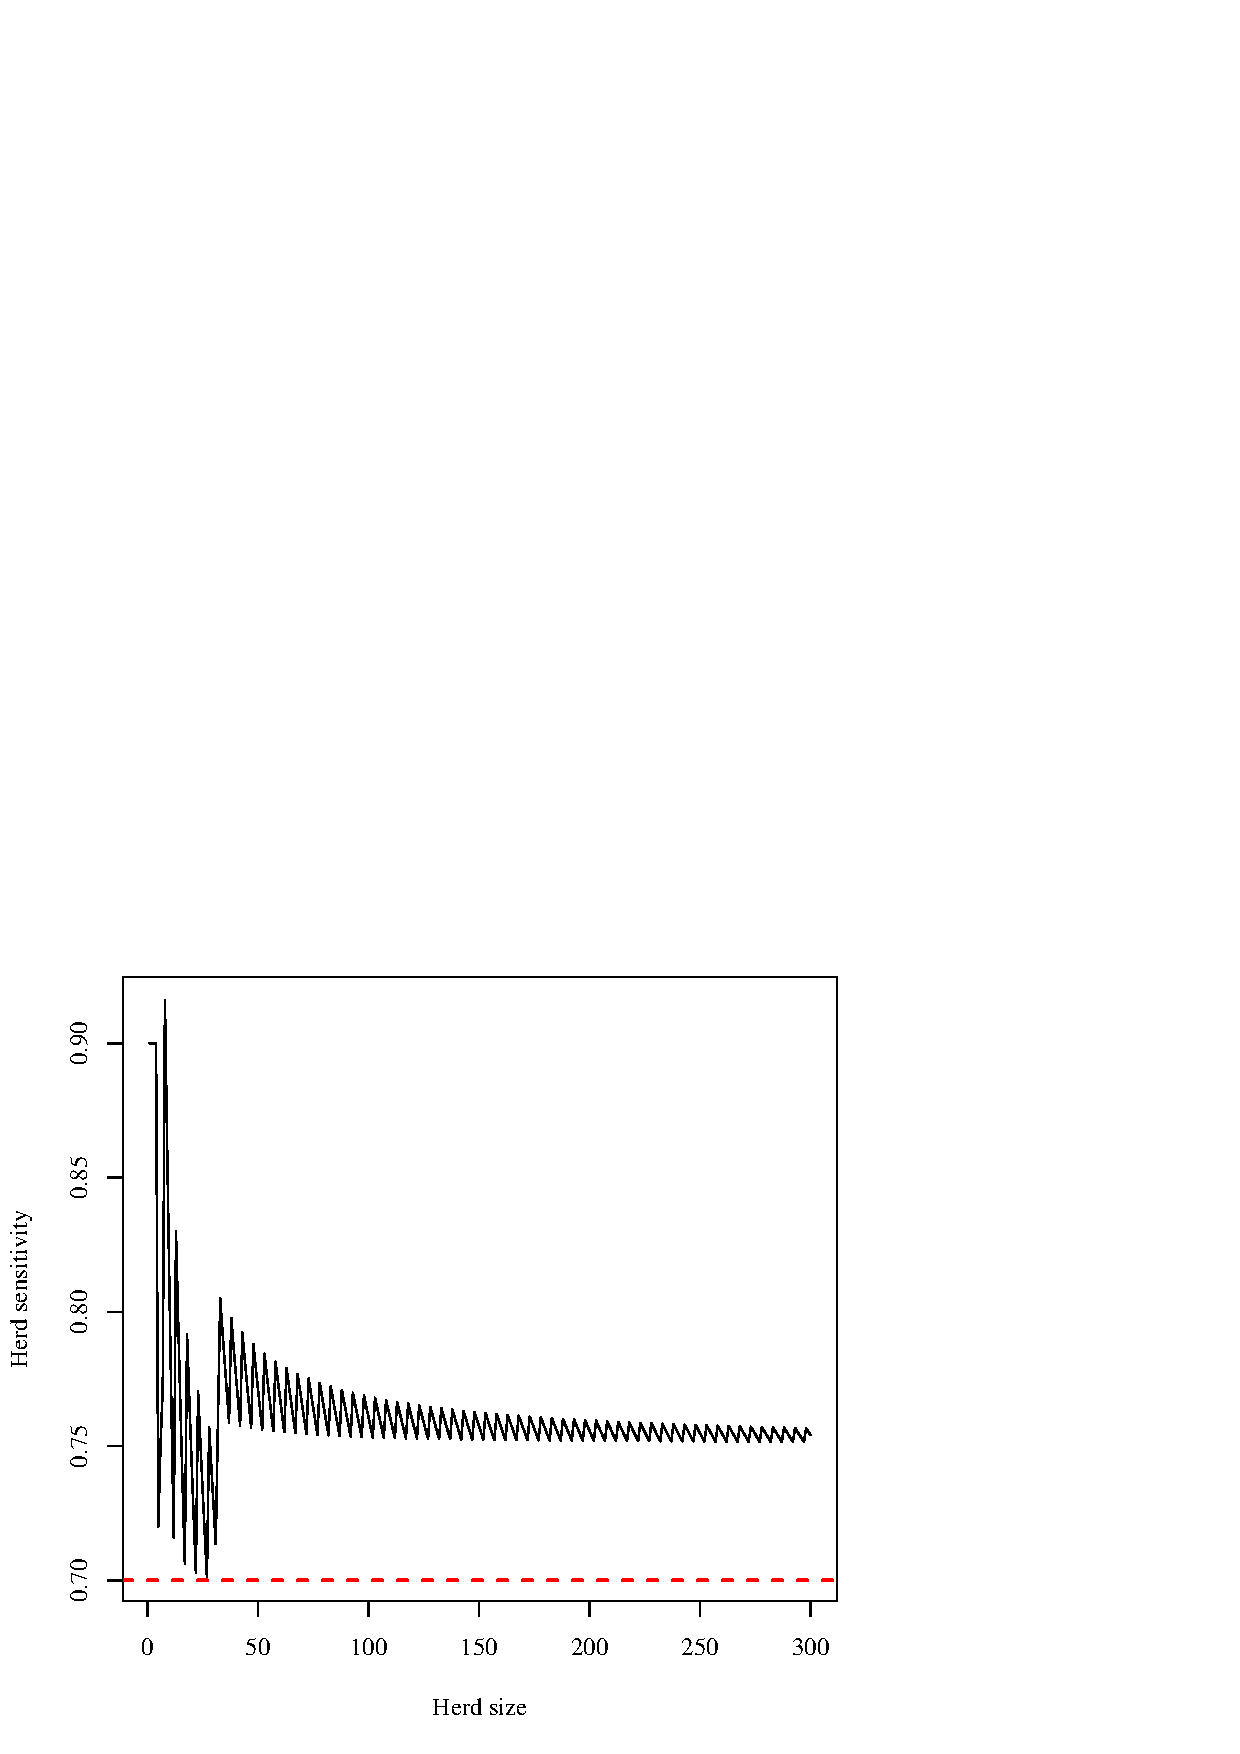
\includegraphics{FFD-intro-003}
\caption{Actually achieved herd sensitivities using individual sampling ($\Se_{herd} = 0.7$, $\pi_{IH} = 0.2$, $\Se_{diag} = 0.9$).}
\label{fig:Herd_sens_ind}
\end{figure}




%%%%%%%%%%%%%%%%%%%%%%%%%%%%%%%%%%%%%%%%%%%%%%%%%%%%%%%%%%%%%%%%%%%%%%%%%%%%%%%

\subsubsection{Limited sampling}
\label{subsubsec:ltd-sampling}
\index{Limited sampling}\index{sampling scheme!limited sampling}

Another strategy used for two-stage sampling is \emph{limited sampling}. With limited sampling, a \textbf{pre-fixed number of animals} $k$ (\emph{sample limit}) \index{sample limit} is tested in each herd, irrespective of the herd size. If the herd has fewer animals then the entire herd is tested. With this approach, the \index{Herd sensitivity} \index{Sensitivity!herd sensitivity} herd sensitivity, i.e., the ability to find a disease in a herd, is no longer constant over the population (as it is for individual sampling), but depends on the herd size. If, e.g., 7 animals are tested out of a herd of 300 then the probability of finding a diseased animal is significantly smaller than when 7 animals are tested out of a herd of 10 animals. Hence, as opposed to individual sampling where the number of animals to test varies over the population, while the herd sensitivity is constant, for limited sampling the opposite is true. The number of animals to test is the same for every herd, but the herd sensitivity varies.

The herd sensitivity $\Se_{herd} = 1 - P(T^+|d)$ can be computed for each herd using (\ref{eq:hypergeom_senspec_T0_simple}), where $N$ is the herd size, $d=N\cdot \pi_{IH}$, $\Se$ is the sensitivity of the diagnostic test \index{Sensitivity!diagnostic sensitivity} \index{Diagnostic sensitivity} and $n=min(N,k)$.

In order to compute the number of herds to be tested using (\ref{eq:hypergeom_senspec_T0_simple}) we, however, require one value for the herd sensitivity and not - as it is the case here - a herd sensitivity depending on the herd size. Hence, the mean herd sensitivity is usually used in the upper-level sample size calculations:

\begin{equation}
%
\Se_{mean} = \sum_{j = 1}^{N_{max}} \Se_{herd}(N=j,k)\cdot P(N=j),
%
\end{equation}

where $N_{max}$ is the biggest herd size in the population, $\Se_{herd}(N=j,k)$ is the herd sensitivity of a herd of size $j$ using limited sampling with a sample limit $k$ and $P(N=j)$ is the proportion of herds with size $j$ in the population, i.e., the ``probability'' that a herd is of size $j$. Using the mean herd sensitivity the number of herds to be tested can again be determined using (\ref{eq:hypergeom_senspec_T0_simple}).

Similar to the herd sensitivity in individual sampling the sample limit determines the balance between the number of animals to test per herd and the number of herds to test, while maintaining a constant \index{Significance level} significance level.


% %%%%%%%%%%%%%%%%%%%%%%%%%%%%%%%%%%%%%%%%%%%%%%%%%%%%%%%%%%%%%%%%%%% %%%%%%%%%%%%%%%%%%%%%%%%%%%%%%%%%%%%%%%%%%%%%%%%%%%%%%%%%%%%%%%%%%% %

\section{A-posteriori calculation of the alpha error} \label{sec:aposteriori}

Recall that the calculation of the sample size on herd level, i.e., the number of herds to test, is based on the herd sensitivity. For limited sampling, the herd sensitivity depends on the size of each herd, hence a mean herd sensitivity is used for the sample size calculation. This, on the other hand, means that the overall significance level of the scheme depends on the chosen sample, i.e., if the sample contains a high proportion of very large herds the mean herd sensitivity in the sample is lower than the mean herd sensitivity in the population and hence the desired overall significance level is not met. If the sample contains a lot of very small herds, then the mean herd sensitivity in the sample exceeds that of the population and the significance of the sampling scheme falls below the desired significance level, i.e., the sampling scheme is ``more thorough'' than necessary.

For individual sampling, on the other hand, we have stated that the number of herds to test is systematically over-estimated, i.e., the actually achieved overall significance of the sampling scheme systematically falls below the desired level, i.e., you are always ``on the safe side''. From a statistical point of view, this poses no problem. It however means that more herds are being tested than necessary and valuable resources are possibly being wasted.

It is therefore of interest to compute the significance level of the sampling scheme after the sample has been drawn, i.e., to compute the \index{A-posteriori alpha error} a-posteriori alpha error, which is the probability of finding no testpositives in the \textbf{given sample}, given that the disease is present at the design prevalence. The a-posteriori alpha error can then be used to assess a given sample and to possibly modify it, i.e., reduce or extend it in order to meet the prescribed significance level.

Let us assume that a specific sample consisting of $n_1$ herds $\{H_1, H_2,\ldots, H_{n_1}\}$ has been chosen. For each herd $H_i$ the corresponding herd sensitivity $\Se_1^{(i)}$ can be computed using (\ref{eq:hypergeom_senspec_T0_simple}). The a-posteriori alpha error is then given by
%
\begin{equation}\label{eq:apost_alpha_exact}
\begin{aligned}
%
\alpha_{apost} &= \sum_{y = \max(0,n_1-N_1+d_1)}^{\min(d_1,n_1)} \frac{{N_1-n_1 \choose d_1-y}}{{N_1 \choose d_1}} \sum_{\big(I\subset \{1,\ldots, n_1\} \wedge |I| = y\big)} \prod_{j\in I} (1-\Se_1^{(j)}),
%
\end{aligned}
\end{equation}
%
where $|I|$ denotes the cardinality, i.e., the number of elements, of the set $I$.

%
%%%%%%%%%%%%%%%%%%%%%%%%%%%%%%%%%%%%%%%%%%%%%%%%%%%%%%%%%%%%%%%%%%% %
\begin{example} \label{ex:a_post_error1}
%
We consider the data \texttt{sheepData} which is included in the package and consists of data from 15287 herds with herd sizes ranging from 1 to 249 animals per herd. Using a significance level of 5~\%, a design prevalence $\pi = 0.002$, an intra-herd prevalence $\pi_{IH} = 0.2$ and a diagnostic sensitivity $\Se = 0.9$. We compute the sample sizes once for individual sampling with a herd sensitivity $\Se_{herd} = 0.7$ and once for limited sampling with a sample limit $k = 7$. Using individual sampling, 2011 herds need to be selected in order to meet a significance level of 5~\%. The mean of the actually achieved herd sensitivity lies at 80.98~\%. Using limited sampling, 1630 herds are required. The sampling scheme yields a mean herd sensitivity of 86.33~\%.

For each of the two sampling schemes, we drew 2000 random samples from the population and computed the a-posteriori alpha errors. The boxplots in Figure~\ref{fig:aPostError_2} illustrate the variability of the a-posteriori error. It can clearly be seen that the error varies around the pre-defined value of 5~\% for limited sampling, and lies below the pre-defined level for individual sampling. %

\begin{figure}[h!t]
\begin{center}
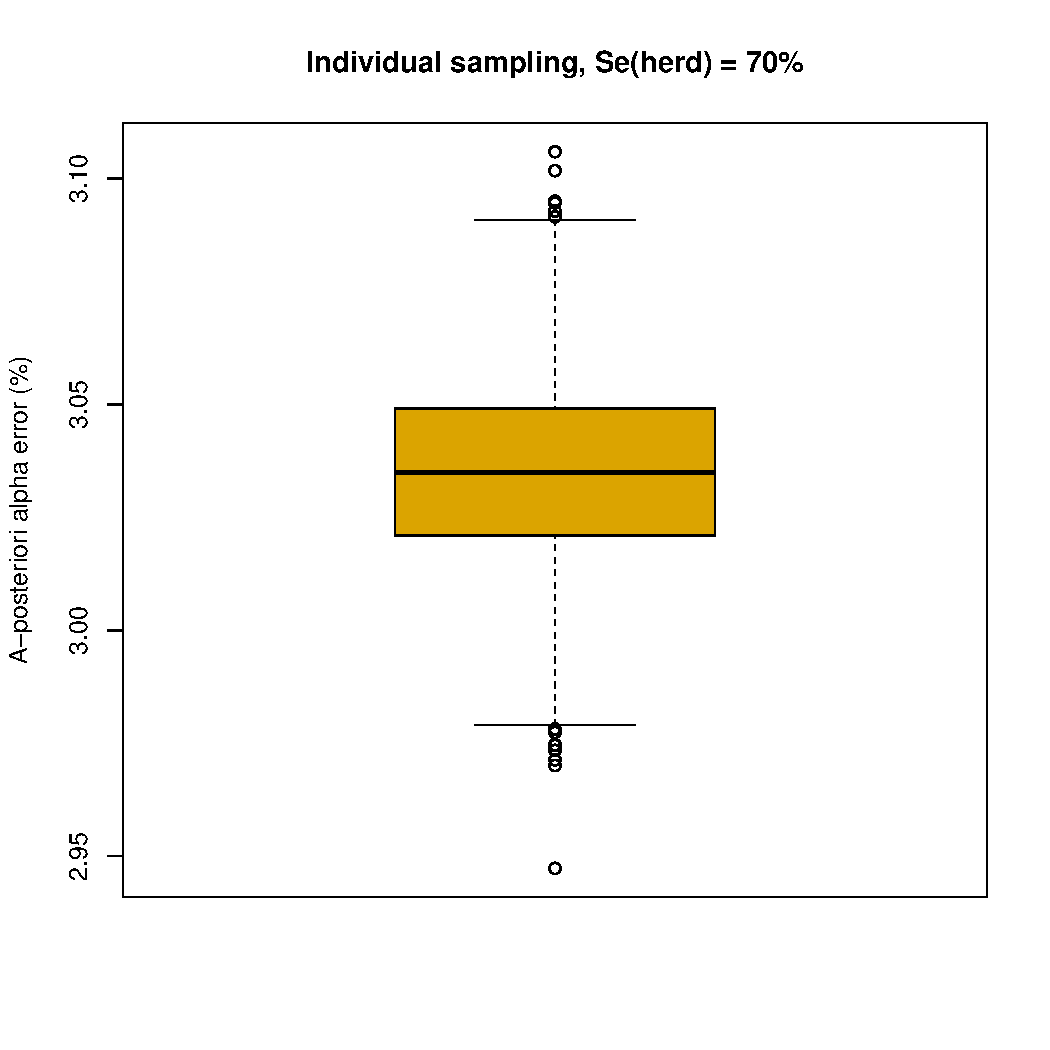
\includegraphics[width=65mm]{aPostError_ind7}\quad 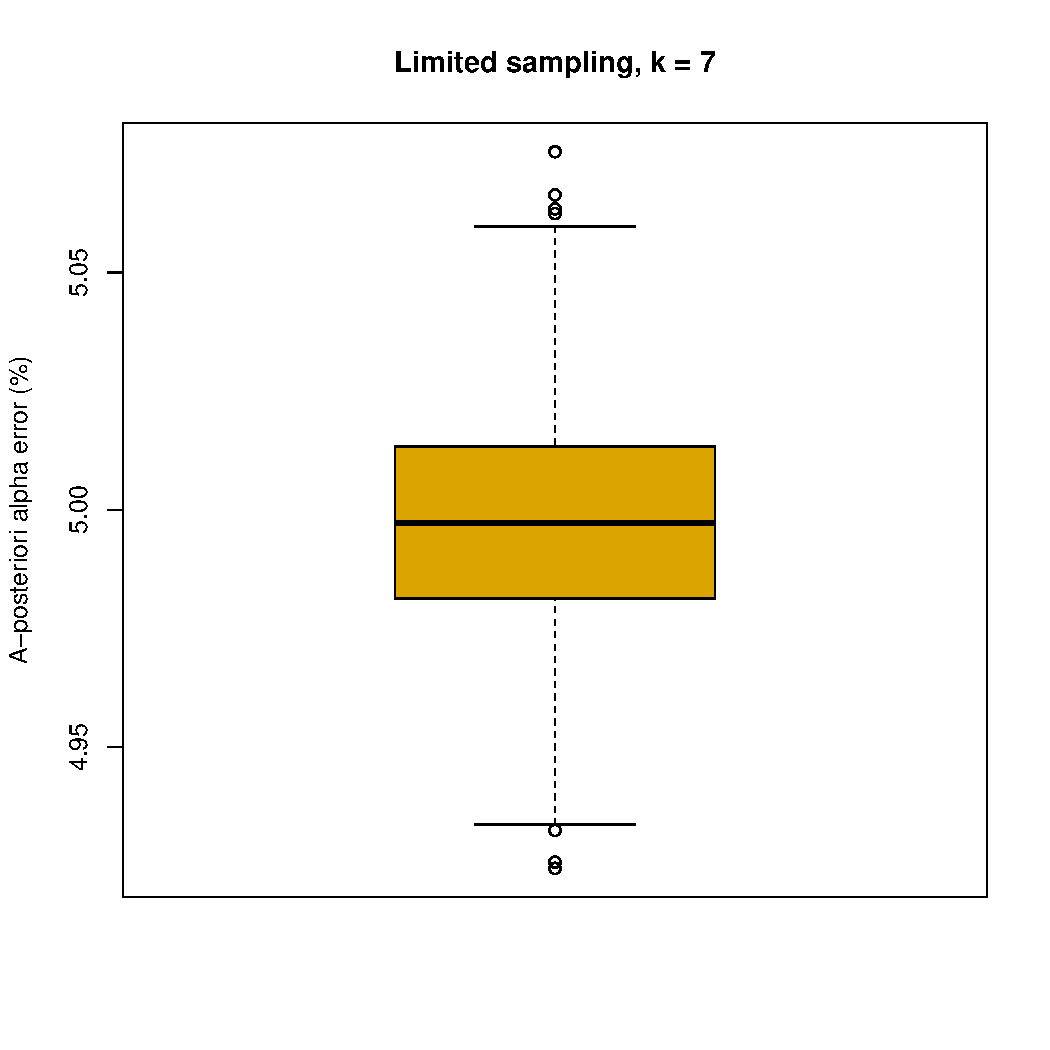
\includegraphics[width=65mm]{aPostError_ltd7}
\end{center}
\caption{Simulated a-posteriori alpha errors for individual sampling with $\Se_{herd} = 0.7$ (left) and limited sampling with $k = 7$ (right).}
\label{fig:aPostError_2}
\end{figure}
%
\end{example}
%
%%%%%%%%%%%%%%%%%%%%%%%%%%%%%%%%%%%%%%%%%%%%%%%%%%%%%%%%%%%%%%%%%%% %

Due to the combinatorial nature of (\ref{eq:apost_alpha_exact}), the evaluation can be challenging. The package \texttt{FFD} offers tools to compute the a-posteriori alpha error for a given sample. Furthermore, a sampling scheme is implemented that updates the a-posteriori alpha error during the sampling procedure and iteratively adds herds to the sample until the desired significance level is met.

% %%%%%%%%%%%%%%%%%%%%%%%%%%%%%%%%%%%%%%%%%%%%%%%%%%%%%%%%%%%%%%%%%%% %%%%%%%%%%%%%%%%%%%%%%%%%%%%%%%%%%%%%%%%%%%%%%%%%%%%%%%%%%%%%%%%%%% %

\section{Risk based sampling} \label{sec:riskbased}

The occurrence of most diseases is influenced by certain external factors, so-called \emph{risk factors}\index{risk factor}. Examples of risk factors associated with animal diseases are the number of animal contacts, import from abroad, distance to the national border, high animal density etc. If the risk associated to the occurrence of a certain risk factor can be quantified, the survey can be made more cost effective by using \emph{risk based surveillance}, i.e., by targeting the sampling on high-risk populations. As the probability of finding a present disease is higher in the high-risk group, the overall sample size can be reduced while still maintaining a constant overall significance level. The package \texttt{FFD} provides methods and functions for the design and the analysis of sampling surveys using categorial risk factors, i.e., where the population can be divided into a finite number of risk groups.

%
%%%%%%%%%%%%%%%%%%%%%%%%%%%%%%%%%%%%%%%%%%%%%%%%%%%%%%%%%%%%%%%%%%% %

\subsection{Two risk groups}

For the sake of clarity we consider a population that is stratified by one dichotomous risk factor, i.e, a population that is divided into two risk groups - a low-risk ($RG_1$) and a high-risk group ($RG_2$). Examples for such a risk factor could be import from abroad (yes/no), animal density (higher/lower than a certain threshold), etc. For these risk groups, the population size $N_1$ and $N_2$ and the risk of contracting the disease $R_1$ and $R_2$, respectively, must be known. In our risk-based survey, we draw a random sample of size $n_1$ from risk group $RG_1$ and a random sample of size $n_2$ from risk group $RG_2$.

%%%%%%%%%%%%%%%%%%%%%%%%%%%%%%%%%%%%%%%%%%%%%%%%%%%%%%%%%%%%%%%%%%%

\subsubsection{The overall alpha error}

According to the design prevalence, we assume that there are $d$ infected herds in the population. If the distribution of the $d$ infected herds among the risk groups is known (i.e., the number of infected herds in $RG_1$ and $RG_2$: $d_1$ and $d_2$ with $d_1+d_2 = d$), the overall alpha error of the risk-based survey can be computed by first computing the alpha error for the individual risk groups
$$
\alpha_i = P(T^+=0 | N_i, n_i, d_i),
$$
using equation \eqref{eq:hypergeom_senspec_T0_simple}, and then multiplying these errors. This becomes clear when we recall that the overall alpha error is the probability of finding no test-positives in the sample, given the disease is present at the design prevalence, which equals the probability of finding no test-positives in risk group $RG_1$ \textbf{and} finding no test-positives in risk group $RG_2$. The distribution of the $d$ diseased herds among the risk groups (i.e., $d_1$ and $d_2$) is, however, not fixed, but a random variable, parameterized by the risk factors $R_i$ and the population sizes $N_i$. To be precise, the number of infected herds in risk group $RG_1$ is binomially distributed with a probability that is proportional to the risk factor $R_1$ and the size of the risk group $N_1$, i.e.,
%
$$d_1 \sim B(d,p_1),$$
%
with
%
\begin{equation}
\label{eq:riskProbability}
p_1 = \frac{R_1N_1}{R_1N_1+R_2N_2}.
\end{equation}
%
Considering this, the overall alpha error can be computed as
%
\begin{align*}
%
P(T^+&=0 | N_1, N_2, n_1, n_2, R_1, R_2, d) = \\
= & \underset{y_1 = \max(0,d-N_2)}{\overset{\min(d,N_1)}{\sum}} {d \choose y_1} p_1^{y_1} \cdot (1-p_1 )^{d-y_1} \cdot
P(T^+=0| N_1,n_1,y_1) \cdot P(T^+=0| N_2,n_2,d-y_1),
%
\end{align*}
%
where again $P(T^+=0| N_i,n_i,d_i)$ is computed using \eqref{eq:hypergeom_senspec_T0_simple}.

\begin{remark}
\begin{enumerate}
\item The probability in \eqref{eq:riskProbability} is invariant to scaling of the risk factors $R_i$, i.e., the value of the probability $p_1$ does not change if the risk factors $R_1,R_2$ are replaced by $\lambda R_1, \lambda R_2$ for any $\lambda \neq 0$. Hence, the exact values of the disease risks $R_i$ need not be specified, only their relative values are of importance. E.g., if the risk of contracting the disease in $RG_2$ is double the risk in $RG_1$ it suffices to set $R_1 = 1$, $R_2 = 2$.
\item The calculation of the overall alpha error above can easily be extended to more than two risk groups by replacing the binomial distribution with a multinomial distribution.
\end{enumerate}
\end{remark}

%%%%%%%%%%%%%%%%%%%%%%%%%%%%%%%%%%%%%%%%%%%%%%%%%%%%%%%%%%%%%%%%%%%

\subsubsection{The optimal sample size}

As before, the optimal sample size is the smallest sample size $n = n_1 + n_2$, satisfying
$$ P(T^+=0 | N_1, N_2, n_1, n_2, R_1, R_2, d)\leq \alpha.$$
If no constraint is set on the distribution of the overall sample size among the risk groups, the minimal sample size is obviously  achieved by sampling only from the group with the highest risk. In many cases such a sample is, however, not desirable. In order to circumvent this issue, appropriate constraints must be defined, eliminating all but one degree of freedom. The package \texttt{FFD} provides two mechanisms, which may be combined to suit the user's needs:
%
\begin{itemize}
%
\item The sample size can be fixed for some risk groups (the sample size for at least one risk group must, however, be left undetermined).
\item For the remaining risk groups weighting factors must be specified. The sample size is then divided among the risk group proportional to the weighting factor $\omega_i$ and the size of the risk group:
    $$n_i = n\cdot \frac{\omega_i N_i}{\sum_j \omega_j N_j}.$$
%
\end{itemize}

% %%%%%%%%%%%%%%%%%%%%%%%%%%%%%%%%%%%%%%%%%%%%%%%%%%%%%%%%%%%%%%%%%%% %%%%%%%%%%%%%%%%%%%%%%%%%%%%%%%%%%%%%%%%%%%%%%%%%%%%%%%%%%%%%%%%%%%
\clearpage

\section{Designing sampling plans using the GUI} \label{sec:using-ffd-GUI}

The most convenient way to use the package \texttt{FFD} is via the \index{GUI} \index{GUI!main window} graphical user interface (GUI). The FFD-GUI is launched by calling the function \verb+FFD_GUI()+ \index{GUI!\verb+FFD_GUI()+} \index{\verb+FFD_GUI()+} in the \proglang{R} console; see Figure~\ref{fig:GUI_reset}. The window is structured into three tabs:

\begin{itemize}
\item \textbf{Data Input:} Specification of the farm data.
\item \textbf{Parameters:} Setting the survey parameters.
\item \textbf{Calculations:} Used for
    \begin{itemize}
    \item sample size calculation, analysis of the overall cost of the survey,
    \item determination of cost-optimal sampling schemes and
    \item sampling from the population.
    \end{itemize}
\end{itemize}


\begin{figure}[h!t]
\begin{center}
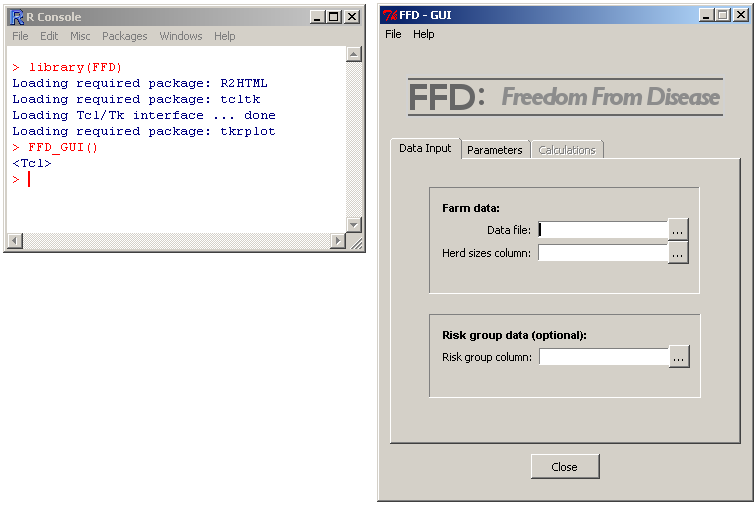
\includegraphics[width=120mm]{GUI_Reset.png}
\end{center}
\caption{Main window of the FFD-GUI}
\label{fig:GUI_reset}
\end{figure}

Via the menu bar settings can be saved and loaded. The file menu further contains built-in examples and help files; see Figure~\ref{fig:GUI_menu}.

\begin{figure}[h!t]
\begin{center}
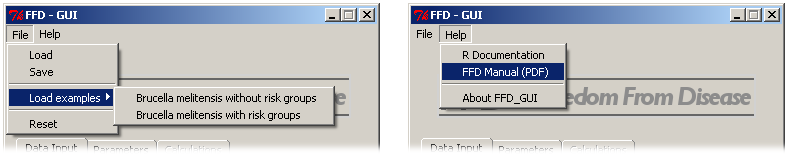
\includegraphics[width=140mm]{GUI_menu.png}
\end{center}
\caption{FFD-GUI menu bar.}
\label{fig:GUI_menu}
\end{figure}

%%%%%%%%%%%%%%%%%%%%%%%%%%%%%%%%%%%%%%%%%%%%%%%%%%%%%%%%%%%%%%%%%%% %%%%%%%%%%%%%%%%%%%%%%%%%%%%%%%%%%%%%%%%%%%%%%%%%%%%%%%%%%%%%%%%%%%
\subsection{Specifying the farm data}
\label{subsec:GUI_farm_data}

In order to compute the herd sensitivities and the first and second stage sample sizes a list of herd sizes of the farms in the population at hand is required. This data is specified in the tab \emph{Data Input} \index{GUI!Data Input} of the GUI. The program requires a data frame with one row per farm and a column containing the herd sizes, i.e. the number of animals on the farm. The data must be provided in the CSV file format, however currently only the central European format with a comma as decimal point and semicolons as column separators is supported. The location of the csv-file is specified in the field \index{GUI!Data File} \emph{Data file}, the name of the column containing the herd size is set in the field \index{GUI!Herd sizes column} \emph{Herd sizes column} via a dropdown menu; see Figure~\ref{fig:GUI_Herd_Size}.

\begin{figure}[h!t]
\begin{center}
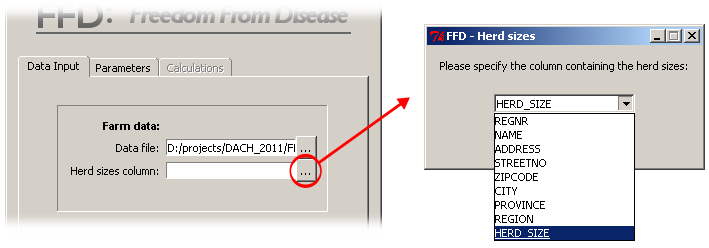
\includegraphics[width=125mm]{GUI_Herd_Size2.png}
\end{center}
\caption{Specifying the farm data.}
\label{fig:GUI_Herd_Size} \end{figure}


%%%%%%%%%%%%%%%%%%%%%%%%%%%%%%%%%%%%%%%%%%%%%%%%%%%%%%%%%%%%%%%%%%% %%%%%%%%%%%%%%%%%%%%%%%%%%%%%%%%%%%%%%%%%%%%%%%%%%%%%%%%%%%%%%%%%%%
\subsection{Setting the survey parameters} \label{subsec:GUI_survey_parameters}

Once the farm data is specified the survey parameters need to be set. Appropriate values for
%
\begin{itemize}
\item the design prevalence,
\item the alpha error,
\item the intra herd prevalence and
\item the test sensitivity
\end{itemize}
%
must be set in the corresponding fields in the tab \index{GUI!Parameters} \emph{Parameters}. Next, the desired sampling strategy (limited sampling or individual sampling) must be chosen in the dropdown menu of the field \index{GUI!Sampling strategy} \emph{Sampling strategy}. The parameters above are necessary for sample size calculations and sensitivity analysis. If additionally, cost analysis and cost optimization is undertaken, the cost per tested animal, as well as the cost per tested herd excluding the costs for the tested animals (e.g., travel costs etc.) must be provided; see Figure~\ref{fig:GUI_Parameters}.

\begin{figure}[h!t]
\begin{center}
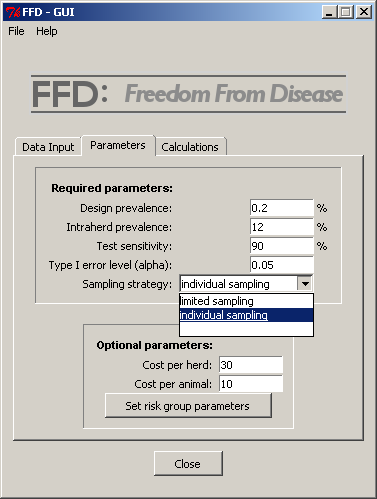
\includegraphics[width=80mm]{GUI_Parameters.png}
\end{center}
\caption{Setting the sampling parameters.} \label{fig:GUI_Parameters}
\end{figure}


%%%%%%%%%%%%%%%%%%%%%%%%%%%%%%%%%%%%%%%%%%%%%%%%%%%%%%%%%%%%%%%%%%% %%%%%%%%%%%%%%%%%%%%%%%%%%%%%%%%%%%%%%%%%%%%%%%%%%%%%%%%%%%%%%%%%%%
\subsection{Sample size and sampling}
\label{subsec:GUI_sample size}

Once a sampling strategy is chosen, the third tab - \index{GUI!Calculations}\emph{Calculations} - becomes accessible. On this tab the actual computations are performed.

\subsubsection{Limited sampling}

For limited sampling the desired \textbf{sample limit} must be specified. A click on the button \emph{Calculate} in the box entitled \emph{Compute sample size} then opens a separate window containing the survey parameters and info on sample sizes on herd and population-level. If information on the sampling costs are provided, then an estimate of the overall cost is given as well; see Figure~\ref{fig:GUI_cald_ltd}. The displayed text can be saved as a text file via the \emph{Save}-button.

\begin{figure}[h!t]
\begin{center}
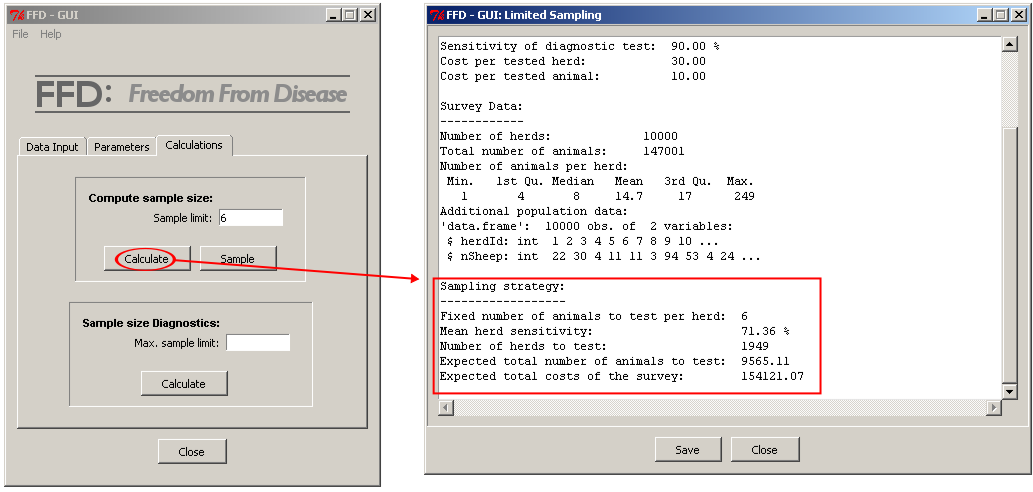
\includegraphics[width=120mm]{GUI_calc_ltd.png}
\end{center}
\caption{Sample sizes for limited sampling.} \label{fig:GUI_cald_ltd}
\end{figure}

A click on the the button \emph{Sample} in the \emph{Compute sample size} box opens a separate window. In this window a strategy regarding the sample size must be specified via a dropdown menu; see Figure~\ref{fig:GUI_sample_ltd1}:

\begin{itemize} \item \textbf{fixed}: The pre-computed sample size (displayed in the info box below) is used. \item \textbf{dynamic}: The alpha error is computed in real time during the sampling process. Farms are added to the sample until the alpha error falls below the specified alpha error-level. \end{itemize}

\begin{figure}[h!t]
\begin{center}
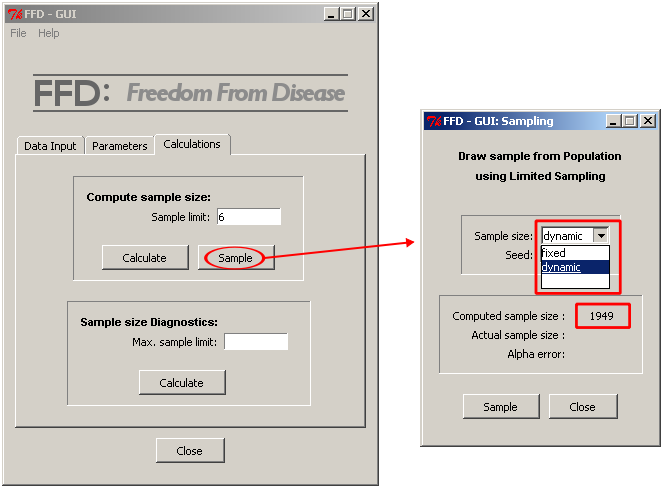
\includegraphics[width=120mm]{GUI_sample_ltd1.png}
\end{center}
\caption{Setting the sample size scheme using individual sampling.} \label{fig:GUI_sample_ltd1}
\end{figure}

In order to allow for reproducibility, an integer valued seed for the random number generator can be set. A click on the the button \emph{Sample} prompts the user to specify a file name. A list of herds is then sampled from the farm list specified in the \emph{Data input}\index{GUI!Data input} tab of the main window and saved as a csv-file to the chosen location (currently only the central European format with a comma as decimal point and semicolons as column separators is supported). Once the sample is drawn, the actual sample size (relevant if dynamic sampling is used) and the actually achieved alpha error are displayed in the info box of the sampling window; see Figure~\ref{fig:GUI_sample_ltd2}.

\begin{figure}[h!t]
\begin{center}
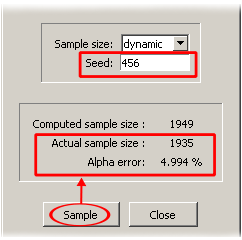
\includegraphics[width=60mm]{GUI_sample_ltd2.png}
\end{center}
\caption{Sampling the farms using individual sampling.} \label{fig:GUI_sample_ltd2}
\end{figure}


\subsubsection{Individual sampling}

For individual sampling the desired \textbf{herd sensitivity} must be specified. A click on the button \emph{Calculate} in the box \emph{Compute sample size} then opens a separate window containing the survey parameters, the number of herds to sample and a lookup table containing the number of animals to sample per herd, depending on the herd size; see Figure~\ref{fig:GUI_calc_ind2}. In case information on the sampling costs are provided an estimate of the overall cost is given as well. The displayed text can be saved as a text file via the \emph{Save}-button.

\begin{figure}[h!t]
\begin{center}
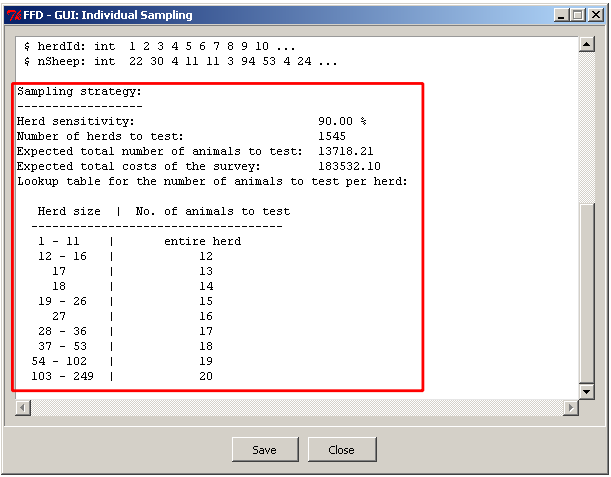
\includegraphics[width=90mm]{GUI_calc_ind2.png}
\end{center} \caption{Sample sizes for individual sampling.} \label{fig:GUI_calc_ind2}
\end{figure}

A click on the the button \emph{Sample} in the \emph{Compute sample size} box opens a separate window. In this window a strategy regarding the sample size must be specified via a dropdown menu (\emph{fixed} or \emph{dynamic}). Additionally, a seed for the random number generator can be specified. A click on the the button \emph{Sample} prompts the user to specify a file name for the sample of farms, which is then saved in the csv-file format. Once the sample is drawn, the actual sample size and the actually achieved alpha error are displayed in the info box of the sampling window.


%%%%%%%%%%%%%%%%%%%%%%%%%%%%%%%%%%%%%%%%%%%%%%%%%%%%%%%%%%%%%%%%%%% %%%%%%%%%%%%%%%%%%%%%%%%%%%%%%%%%%%%%%%%%%%%%%%%%%%%%%%%%%%%%%%%%%%
\subsection{Survey diagnostics}
\label{subsec:GUI_cost_analysis}

In the field \emph{Sample size diagnostics}\index{GUI!Sample size diagnostics} on the \emph{Calculations} tab the overall costs of the survey, as well as the herd sensitivity, the number of herds to test and the overall number of animals to test are estimated for a range of sample limits (limited sampling) or herd sensitivities (individual sampling), respectively. The results are displayed in forms of graphs and the cost optimal value for the sample limit or herd sensitivity, respectively, is determined.

For limited sampling the maximal sample limit must be provided. The above mentioned figures are then computed for all sample limits between 1 and the maximal sample limit, i.e., for a maximal sample limit of 5, the sample sizes and overall costs are computed for sample limits of 1,2,3,4 and 5.

For individual sampling a step size for the herd sensitivity must be specified. The above mentioned figures are then computed for herd sensitivities ranging between 10~\% and the specified sensitivity of the diagnostic test (as this is the maximally achievable herd sensitivity if all animals are tested in a herd with one infected animal), using the specified step size, e.g., for a herd sensitivity of 90~\% and a step size of 5~\%, the sample sizes and overall costs are computed for herd sensitivities of 10~\%, 15~\%,$\ldots$, 85~\%, 90~\%.

A click on the button \emph{Calculate} in the \emph{Sample size diagnostics} field opens a separate window containing the survey parameters, sample sizes and herd sensitivity for the cost optimal survey (Figure~\ref{fig:GUI_diag_ltd1}). The displayed text can be saved as a text file via the \emph{Save}-button.

\begin{figure}[h!t]
\begin{center}
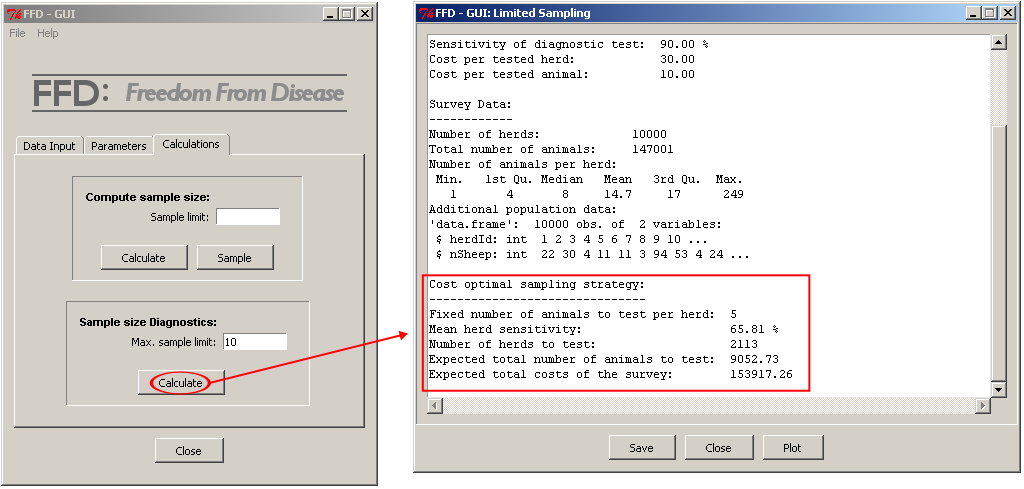
\includegraphics[width=120mm]{GUI_diag_ltd1.png}
\end{center}
\caption{Sample size diagnostics for limited sampling.} \label{fig:GUI_diag_ltd1}
\end{figure}

A click on the \emph{Plot} button produces a graphic containing 4 plots:
%
\begin{itemize}
\item the mean herd sensitivity against the sample limit,
\item the number of herds to test against the sample limit,
\item the expected total number of animals to test against the sample limit and
\item the expected total costs of the survey against the sample limit
\end{itemize}
%
for limited sampling (Figure~\ref{fig:GUI_diag_ltd2}) and
%
\begin{itemize}
\item the mean number of animals to test per herd against the herd sensitivity,
\item the number of herds to test against the herd sensitivity,
\item the expected total number of animals to test against the herd sensitivity and
\item the expected total costs of the survey against the herd sensitivity
\end{itemize}
%
for individual sampling. These plots can be saved as .jpg, .png or .pdf graphics via the button \emph{Save}.

\begin{figure}[h!t]
\begin{center}
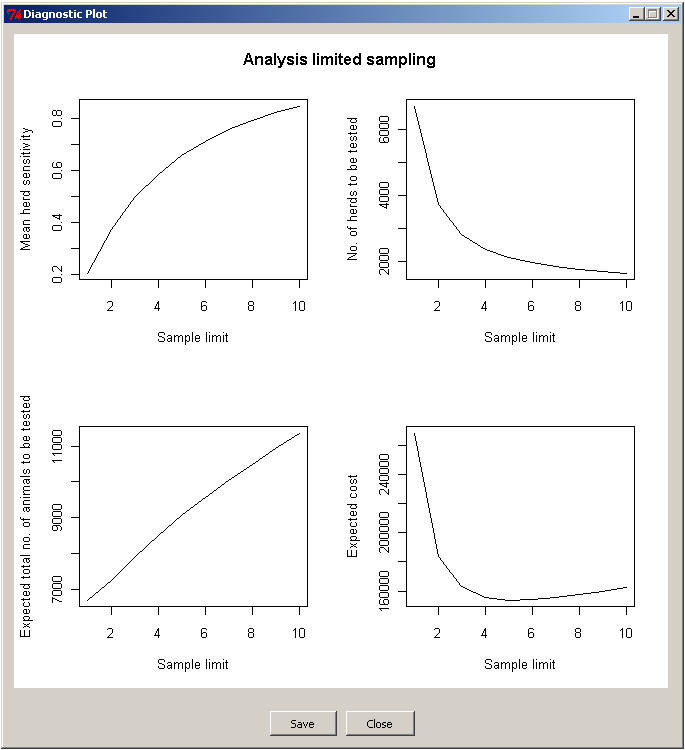
\includegraphics[width=90mm]{GUI_diag_ltd2.png}
\end{center}
\caption{Diagnostic plots for limited sampling.} \label{fig:GUI_diag_ltd2}
\end{figure}


%%%%%%%%%%%%%%%%%%%%%%%%%%%%%%%%%%%%%%%%%%%%%%%%%%%%%%%%%%%%%%%%%%% %%%%%%%%%%%%%%%%%%%%%%%%%%%%%%%%%%%%%%%%%%%%%%%%%%%%%%%%%%%%%%%%%%%
\subsection{Risk based sampling}
\label{subsec:GUI_riskBased}

In order to perform risk based sampling, a vector stating the risk group that each farm falls into must be specified. This data must be contained as a separate column in the data frame that was specified in the tab \emph{Data Input} \index{GUI!Data Input} in the field \index{GUI!Data File} \emph{Data file}. The name of the column containing the risk group affiliation is set in the field \index{GUI!Risk group column} \emph{Risk group column} via a dropdown menu; see Figure~\ref{fig:GUI_Risk_Group}.

\begin{figure}[h!t]
\begin{center}
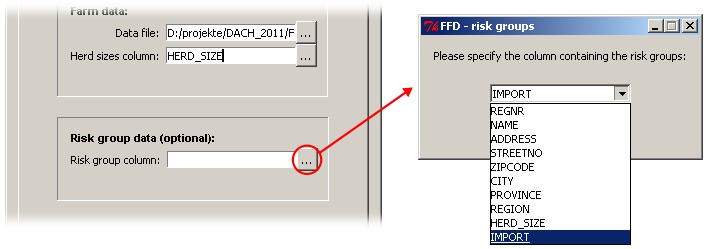
\includegraphics[width=125mm]{GUI_Risk_Group.png}
\end{center}
\caption{Specifying the risk groups that each farm belongs to (tab: Data input).}
\label{fig:GUI_Risk_Group} \end{figure}

In the next step, the (relative) disease risks associated to the specified risk groups must be set. This is done in the tab \emph{Parameters} \index{GUI!Parameters} by clicking on \index{GUI!Set risk group parameters} \emph{Set risk group parameters} in the field \index{GUI!Optional parameters} \emph{Optional parameters}; see Figure~\ref{fig:GUI_Risk_Data}.

\begin{figure}[h!t]
\begin{center}
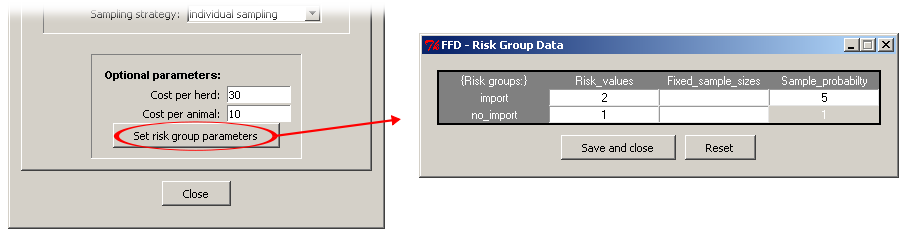
\includegraphics[width=125mm]{GUI_Risk_Data.png}
\end{center}
\caption{Specifying the relative risks and parameters for the sample size distribution among the risk groups (tab: Parameters).}
\label{fig:GUI_Risk_Data} \end{figure}

A click on the button \emph{Set risk group parameters} opens a separate data input matrix. The risk groups make up the rows, the disease risks are entered in the first column, entitled \emph{Risk\_values} \index{GUI!Risk\_values}.

For the computation of the optimal sample size, the user must specify \textbf{exactly one} of two parameters for each risk group:
%
\begin{itemize}
\item a fixed sample size (column \emph{Fixed\_sample\_sizes} \index{GUI!Fixed\_sample\_sizes}) or
\item a weighting factor (column \emph{Sample\_probability} \index{GUI!Sample\_probability}).
\end{itemize}
%

If all the parameters are correctly specified, sample size calculation, sampling and survey diagnostics can be performed same as for non-targeted sampling. E.g., a click on the button \emph{Calculate} in the box \emph{Compute sample size} on tab \emph{Calculations} will promt the user to choose between risk-based and non-targeted sampling. If risk-based sampling is selected, the total sample size is returned, as well as the sample size for each risk group; see Figure~\ref{fig:GUI_calc_ind_risk}.

\begin{figure}[h!t]
\begin{center}
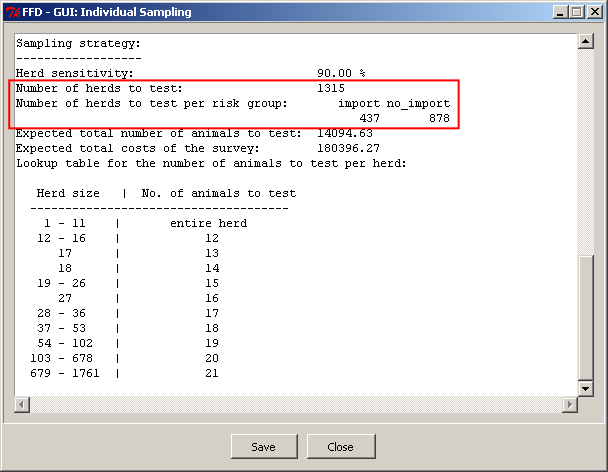
\includegraphics[width=90mm]{GUI_calc_ind_risk.png}
\end{center} \caption{Sample sizes for risk-based individual sampling.} \label{fig:GUI_calc_ind_risk}
\end{figure}

% %%%%%%%%%%%%%%%%%%%%%%%%%%%%%%%%%%%%%%%%%%%%%%%%%%%%%%%%%%%%%%%%%%% %%%%%%%%%%%%%%%%%%%%%%%%%%%%%%%%%%%%%%%%%%%%%%%%%%%%%%%%%%%%%%%%%%% %
\clearpage

\section{Sample size calculation using S4 classes} %\section{FFD using the S4 classes and methods}
\label{sec:using-ffd-S4}

The package \texttt{FFD} offers convenient tools to compute the sample sizes on herd and on animal level for individual and limited sampling using S4-classes. With these classes the survey parameters need to be specified once, creating an object of the class \texttt{SurveyData}. With this object different sampling strategies can conveniently be compared with respect to effectivity and costs and appropriate strategies can be evaluated and exported as html-files.

Furthermore, functions are available to evaluate (\ref{eq:hypergeom_senspec_T0_simple}), find the optimal sample sizes on herd and animal level, to evaluate herd sensitivities for limited sampling etc. These functions operate with conventional R-classes (vectors, data frames) and, while the use is not as convenient as with the methods for the S4 classes, they offer a greater flexibility.

%%%%%%%%%%%%%%%%%%%%%%%%%%%%%%%%%%%%%%%%%%%%%%%%%%%%%%%%%%%%%%%%%%%

\subsection{Specifying the survey parameters} \label{subsec:surveyData}

The following parameters/data are required in order to fix the sample size:

\begin{itemize}
%
\item \texttt{nAnimalVec}: A vector of herd sizes (=number of animals in a herd). Each component of the vector  corresponds to a herd in the population,
\item \texttt{designPrevalence}: The prevalence threshold in the population that the survey must establish,
\item \texttt{alpha}: Significance level of the survey (= 1 - confidence),
\item \texttt{intraHerdPrevalence}: The assumed prevalence of the disease within an infected herd,
\item \texttt{diagSensitivity}: The sensitivity of the diagnostic test.
%
\end{itemize}

If it is desired to optimize the sampling strategy with respect to overall costs, parameters \texttt{costHerd}, \texttt{costAnimal}, describing the cost of each tested herd (excluding the cost per tested animal) and the cost of each tested animal, respectively. The overall costs are then computed using the simple model:

$$\mbox{cost = number of tested herds * cost per herd + number of tested animals * cost per animal}.$$

The cost per tested animal, e.g., contain the cost of drawing and analyzing the sample. The cost per tested herd could contain the travel costs of the vet etc.

All the survey parameters are packed into an S4 object of the class \texttt{SurveyData} \index{Class!\texttt{SurveyData}} \index{\texttt{SurveyData}}  using the constructor \texttt{surveyData()}. \index{\texttt{surveyData()}} Additionally, further population data, such as herd identifiers, names and addresses of the owners etc. can be passed to the constructor in the form of a data frame, where each row of the data frame corresponds to a component of the vector \texttt{nAnimalVec}.

In the following example the data set \texttt{sheepData}, contained in the package \texttt{FFD}, is used. The data set contains simulated data resembling the sheep holdings in Austria.



\begin{Schunk}
\begin{Sinput}
> data(sheepData)
> mySurvey <- surveyData(nAnimalVec = sheepData$nSheep,
       populationData = sheepData, designPrevalence = 0.002,
       alpha = 0.05, intraHerdPrevalence = 0.2,
       diagSensitivity = 0.9, costHerd = 30, costAnimal = 7)
> summary(mySurvey)
\end{Sinput}
\begin{Soutput}
 Survey Parameters:                             
 ------------------                             
 Design Prevalence:               0.002         
 Significance level:              0.05          
 Intra herd prevalence:           0.200         
 Sensitivity of diagnostic test:  0.900         
 Cost per tested herd:            30.00         
 Cost per tested animal:          7.00          
                                                
 Survey Data:                                   
 ------------                                   
 Number of herds:             15287             
 Total number of animals:     224606            
 Number of animals per herd:                    
  Min.   1st Qu. Median   Mean   3rd Qu.  Max.  
    1       4       8     14.69    17      249  
 No risk group data.                            
 No risk value data.                            
 Additional population data:                    
 'data.frame':  15287 obs. of  3 variables:     
  $ herdId: int  1 2 3 4 5 6 7 8 9 10 ...       
  $ state : int  7 7 6 3 8 7 3 7 4 3 ...        
  $ nSheep: num  22 30 4 11 11 3 94 53 4 24 ... 
\end{Soutput}
\end{Schunk}

\index{Method!\texttt{summary-SurveyData}} \index{Method!\texttt{show-SurveyData}} Objects of the class \texttt{SurveyData} are the basic building blocks used in the package \texttt{FFD}, containing all the necessary data for the design of an appropriate sampling scheme using individual or limited sampling.

%%%%%%%%%%%%%%%%%%%%%%%%%%%%%%%%%%%%%%%%%%%%%%%%%%%%%%%%%%%%%%%%%%%

\subsection{Individual sampling} \label{subsec:ind-sampling}

With individual sampling the number of animals to test per herd in order to achieve a specified herd sensitivity depends on the herd size. The herd sensitivity, hence, determines the number of animals to test per herd, as well as the number of herd to test, while maintaining a constant overall significance level $\alpha$. If a low herd sensitivity is chosen the number of animals to test per herd is low, while the number of herds to test might be rather high. If, however a high herd sensitivity is specified the number of animals tested per herd increases, while the number of herds to test decreases. If the cost per tested herd and the cost per tested animal is known a herd sensitivity might be chosen in order to minimize the overall costs of the survey.

\subsubsection{Cost optimization}

The package \texttt{FFD} provides the S4-class \texttt{IndSamplingSummary} \index{Class!\texttt{IndSamplingSummary}} \index{\texttt{IndSamplingSummary}} and the function \texttt{indSamplingSummary()}, \index{\texttt{indSamplingSummary()}} as a convenient tool to minimize the survey costs for individual sampling. The class constructor \texttt{indSamplingSummary()} takes an object of the class \texttt{SurveyData} and a step size for the herd sensitivities as an argument and computes the number of herds to test, the expected total number of animals tested based on the herd size distribution in the population, as well as the expected overall costs of the survey for a sequence of herd sensitivities. The herd sensitivities range from 0.1 to the sensitivity of the diagnostic test, the step size for the discretization is either specified by the user or a default value of 0.02 is used.

\begin{Schunk}
\begin{Sinput}
> myIndSamplingSummary <- indSamplingSummary(survey.Data = mySurvey,
       stepSize = 0.05)
> summary(myIndSamplingSummary)
\end{Sinput}
\begin{Soutput}
 INDIVIDUAL SAMPLING DIAGNOSTICS:                    
                                                     
 Survey Parameters:                                  
 ------------------                                  
 Design Prevalence:               0.002              
 Significance level:              0.05               
 Intra herd prevalence:           0.200              
 Sensitivity of diagnostic test:  0.900              
 Cost per tested herd:            30.00              
 Cost per tested animal:          7.00               
                                                     
 Survey Data:                                        
 ------------                                        
 Number of herds:             15287                  
 Total number of animals:     224606                 
 Number of animals per herd:                         
  Min.   1st Qu. Median   Mean   3rd Qu.  Max.       
    1       4       8     14.69    17      249       
 No risk group data.                                 
 No risk value data.                                 
 Additional population data:                         
 'data.frame':  15287 obs. of  3 variables:          
  $ herdId: int  1 2 3 4 5 6 7 8 9 10 ...            
  $ state : int  7 7 6 3 8 7 3 7 4 3 ...             
  $ nSheep: num  22 30 4 11 11 3 94 53 4 24 ...      
                                                     
 Cost optimal sampling strategy:                     
 -------------------------------                     
 Herd sensitivity:                          0.900    
 Number of herds to test:                   1564     
 Expected total number of animals to test:  10743.38 
 Expected total costs of the survey:        122123.67
\end{Soutput}
\end{Schunk}

\index{Method!\texttt{summary-IndSamplingSummary}} \index{Method!\texttt{show-IndSamplingSummary}} A plot of the object of class \texttt{IndSamplingSummary} can be created using \texttt{plot()}. \index{Method!\texttt{plot-IndSamplingSummary}} The plot consists of (row-wise from top left to bottom right)

\begin{itemize}
\item the mean number of animals to test per herd plotted against the herd sensitivity,
\item the number of herds to test plotted against the herd sensitivity,
\item the expected total number of animals to test plotted against the herd sensitivity,
\item the expected overall costs plotted against the herd sensitivity.
\end{itemize}

\setkeys{Gin}{width=15cm}
\begin{Schunk}
\begin{Sinput}
> plot(myIndSamplingSummary)
\end{Sinput}
\end{Schunk}
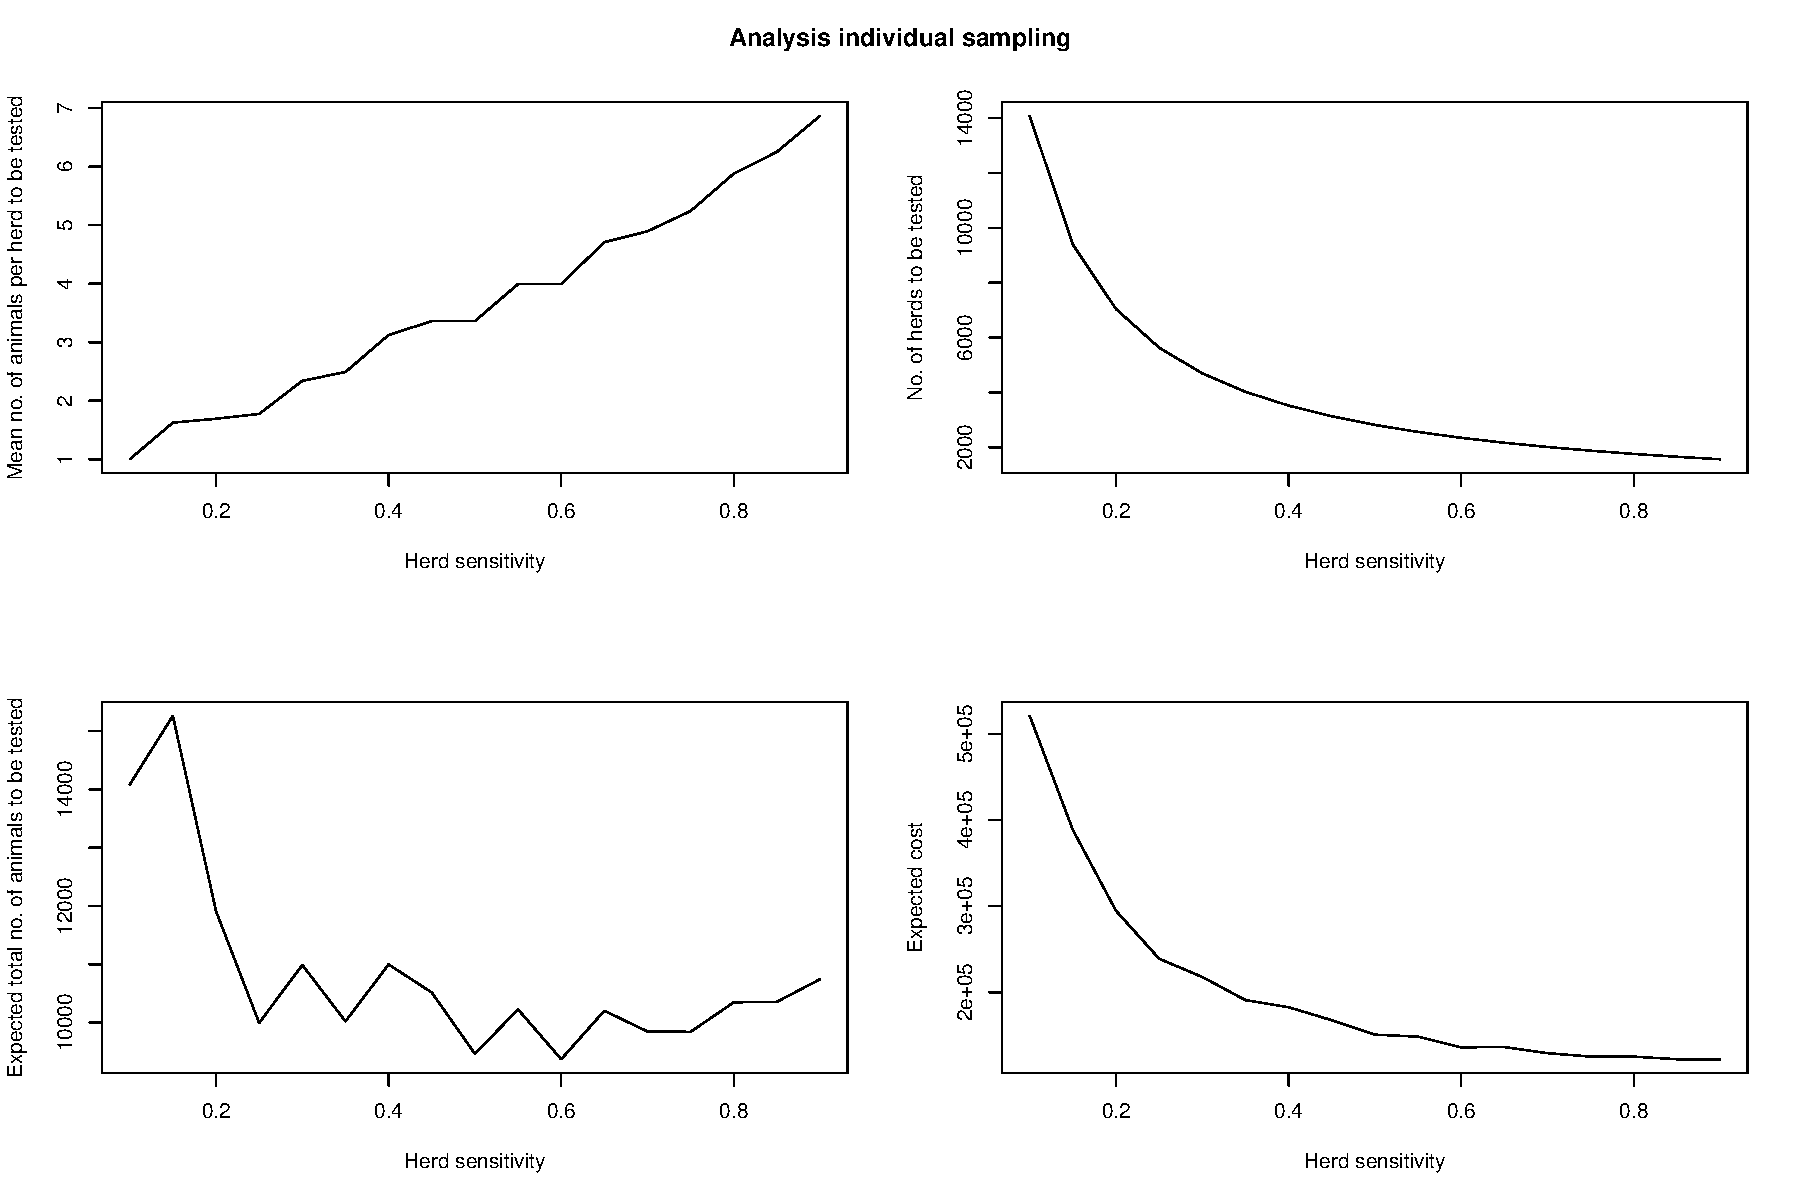
\includegraphics{FFD-intro-006}

The summary of the object of class \texttt{IndSamplingSummary} can further be exported to an html-file using the method \texttt{HTML}. \index{Method!\texttt{HTML-IndSamplingSummary}} This method creates an html-file and a css-file containing the the data in the \texttt{IndSamplingSummary} object, as well as the diagnostic plots.

\begin{Schunk}
\begin{Sinput}
> HTML(myIndSamplingSummary)
\end{Sinput}
\end{Schunk}

The method further accepts the same arguments as the function \texttt{HTMLInitFile()} from the package \texttt{R2HTML}, e.g., \texttt{filename}, \texttt{outdir}, \texttt{CSSFile} and \texttt{Title}.


\subsubsection{Parameters for a fixed herd sensitivity}

If one has decided on an appropriate herd sensitivity, number of herds to test, the expected total number of animals to test, the expected costs and a lookup table containing the number of animals to test per herd depending on the herd size can be computed using the function \texttt{indSampling()} \index{\texttt{indSampling()}} to create an object of the class \texttt{IndSampling}. \index{Class!\texttt{IndSampling}} \index{\texttt{IndSampling}} The function takes two arguments, \texttt{survey.Data}, an object of the class \texttt{SurveyData}, and the herd sensitivity \texttt{herdSensitivity}. The computed parameters can again be displayed using the methods \texttt{show()}, \texttt{summary()} and \texttt{HTML()}. \index{Method!\texttt{show-IndSampling}} \index{Method!\texttt{summary-IndSampling}} \index{Method!\texttt{HTML-IndSampling}}

For a herd sensitivity of 0.7 the parameters are:

\begin{Schunk}
\begin{Sinput}
> myIndSampling <- indSampling(survey.Data = mySurvey,
       herdSensitivity = 0.7)
> summary(myIndSampling)
\end{Sinput}
\begin{Soutput}
 INDIVIDUAL SAMPLING:                                    
                                                         
 Survey Parameters:                                      
 ------------------                                      
 Design Prevalence:               0.002                  
 Significance level:              0.05                   
 Intra herd prevalence:           0.200                  
 Sensitivity of diagnostic test:  0.900                  
 Cost per tested herd:            30.00                  
 Cost per tested animal:          7.00                   
                                                         
 Survey Data:                                            
 ------------                                            
 Number of herds:             15287                      
 Total number of animals:     224606                     
 Number of animals per herd:                             
  Min.   1st Qu. Median   Mean   3rd Qu.  Max.           
    1       4       8     14.69    17      249           
 No risk group data.                                     
 No risk value data.                                     
 Additional population data:                             
 'data.frame':  15287 obs. of  3 variables:              
  $ herdId: int  1 2 3 4 5 6 7 8 9 10 ...                
  $ state : int  7 7 6 3 8 7 3 7 4 3 ...                 
  $ nSheep: num  22 30 4 11 11 3 94 53 4 24 ...          
                                                         
 Sampling strategy:                                      
 ------------------                                      
 Herd sensitivity:                          0.700        
 Number of herds to test:                   2011         
 Expected total number of animals to test:  9845.44      
 Expected total costs of the survey:        129248.09    
 Lookup table for the number of animals to test per herd:
                                                         
    Herd size  |  No. of animals to test                 
   ------------------------------------                  
     1 - 3    |       entire herd                        
     4 - 5    |            4                             
       6      |            5                             
    7 - 31    |            6                             
   32 - 249   |            7                             
\end{Soutput}
\end{Schunk}

%%%%%%%%%%%%%%%%%%%%%%%%%%%%%%%%%%%%%%%%%%%%%%%%%%%%%%%%%%%%%%%%%%%

\subsection{Limited sampling} \label{subsec:ltd-sampling}

For limited sampling a pre-fixed number of animals per selected herd (=the sample limit) is tested, irrespective of the actual herd size. The chosen sample limit determines the (mean) herd sensitivity and thus the sample size on a herd level. The sample limit and the number of herds act in a complementary fashion in the sense that low sampling limits result in a large number of herds to be tested and vice versa. If the cost per tested herd and the cost per tested animal is known the package can be used to find the cost optimal sample limit.

\subsubsection{Cost optimization}

The package \texttt{FFD} provides the S4-class \texttt{LtdSamplingSummary} \index{Class!\texttt{LtdSamplingSummary}} \index{\texttt{LtdSamplingSummary}} and the function \texttt{ltdSamplingSummary()}, \index{\texttt{ltdSamplingSummary()}} where the mean herd sensitivity, the number of herds to test, the expected total number of animals tested based on the herd size distribution in the population, as well as the expected overall costs of the survey is computed for a sequence of sample limits. The smallest considered sample limit is 1 animal per herd, the largest sample limit can be specified by the user via the argument \texttt{sampleSizeLtdMax}, or if no upper bound is specified, the largest herd size is used.

\begin{Schunk}
\begin{Sinput}
> myLtdSampleSummary <- ltdSamplingSummary(survey.Data = mySurvey,
       sampleSizeLtdMax = 30)
> summary(myLtdSampleSummary)
\end{Sinput}
\begin{Soutput}
 LIMITED SAMPLING DIAGNOSTICS:                       
                                                     
 Survey Parameters:                                  
 ------------------                                  
 Design Prevalence:               0.002              
 Significance level:              0.05               
 Intra herd prevalence:           0.200              
 Sensitivity of diagnostic test:  0.900              
 Cost per tested herd:            30.00              
 Cost per tested animal:          7.00               
                                                     
 Survey Data:                                        
 ------------                                        
 Number of herds:             15287                  
 Total number of animals:     224606                 
 Number of animals per herd:                         
  Min.   1st Qu. Median   Mean   3rd Qu.  Max.       
    1       4       8     14.69    17      249       
 No risk group data.                                 
 No risk value data.                                 
 Additional population data:                         
 'data.frame':  15287 obs. of  3 variables:          
  $ herdId: int  1 2 3 4 5 6 7 8 9 10 ...            
  $ state : int  7 7 6 3 8 7 3 7 4 3 ...             
  $ nSheep: num  22 30 4 11 11 3 94 53 4 24 ...      
                                                     
 Cost optimal sampling strategy:                     
 -------------------------------                     
 Fixed number of animals to test per herd:  5        
 Mean herd sensitivity:                     0.769    
 Number of herds to test:                   1830     
 Expected total number of animals to test:  7854.38  
 Expected total costs of the survey:        109880.68
\end{Soutput}
\end{Schunk}

\index{Method!\texttt{summary-LtdSamplingSummary}} \index{Method!\texttt{show-LtdSamplingSummary}} A plot of the object of class \texttt{LtdSamplingSummary} can be created using \texttt{plot()}. \index{Method!\texttt{plot-LtdSamplingSummary}} The plot consists of (row-wise from top left to bottom right)

\begin{itemize}
\item the mean herd sensitivity plotted against the sample limit,
\item the number of herds to test plotted against the sample limit,
\item the expected total number of animals to test plotted against the sample limit,
\item the expected overall costs plotted against the sample limit.
\end{itemize}

\setkeys{Gin}{width=15cm}
\begin{Schunk}
\begin{Sinput}
> plot(myLtdSampleSummary)
\end{Sinput}
\end{Schunk}
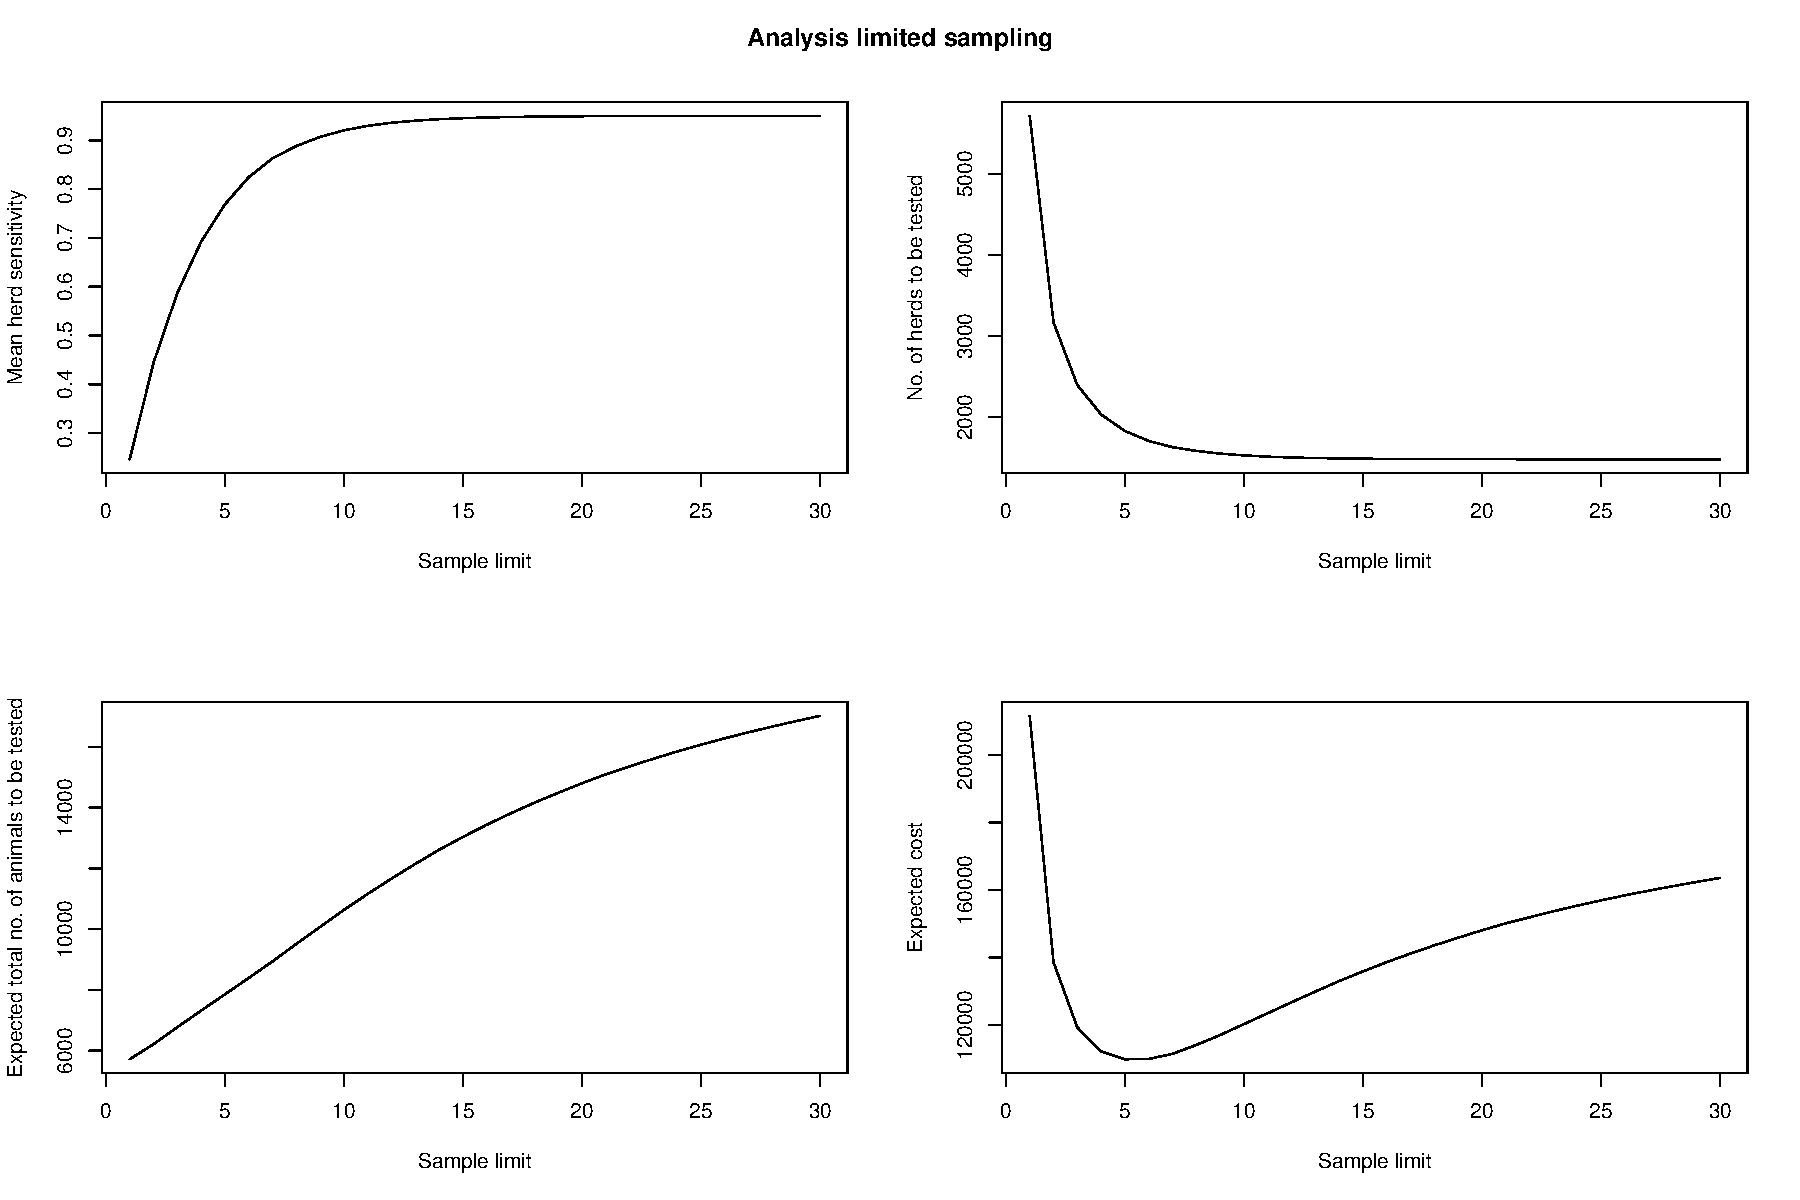
\includegraphics{FFD-intro-009}

The summary of the object of class \texttt{LtdSamplingSummary} can further be exported to an html-file using the method \texttt{HTML}. \index{Method!\texttt{HTML-LtdSamplingSummary}} This method creates an html-file and a css-file containing the the data in the \texttt{IndSamplingSummary} object, as well as the diagnostic plots.


\begin{Schunk}
\begin{Sinput}
> HTML(myLtdSamplingSummary)
\end{Sinput}
\end{Schunk}

The method further accepts the same arguments as the function \texttt{HTMLInitFile()} from the package \texttt{R2HTML}, e.g., \texttt{filename}, \texttt{outdir}, \texttt{CSSFile} and \texttt{Title}.

\subsubsection{Parameters for a fixed sample limit}

If one has decided on an appropriate sample size the herd sensitivity, number of herds to test, expected total number of animals to test and expected costs can be determined using the function \texttt{ltdSampling()} \index{\texttt{ltdSampling()}} to create an object of the class \texttt{LtdSampling}. \index{Class!\texttt{LtdSampling}} \index{\texttt{LtdSampling}} The function takes two arguments, \texttt{survey.Data}, an object of the class \texttt{SurveyData}, and the sample limit \texttt{sampleSizeLtd}. The computed parameters can again be displayed using the methods \texttt{show()}, \texttt{summary()} and \texttt{HTML()}. \index{Method!\texttt{show-LtdSampling}} \index{Method!\texttt{summary-LtdSampling}} \index{Method!\texttt{HTML-LtdSampling}}

Let's say we have chosen the appropriate sample limit to be 7 animals per herd:

\begin{Schunk}
\begin{Sinput}
> myLtdSampling <- ltdSampling(survey.Data = mySurvey, sampleSizeLtd = 7)
> summary(myLtdSampling)
\end{Sinput}
\begin{Soutput}
 LIMITED SAMPLING:                                   
                                                     
 Survey Parameters:                                  
 ------------------                                  
 Design Prevalence:               0.002              
 Significance level:              0.05               
 Intra herd prevalence:           0.200              
 Sensitivity of diagnostic test:  0.900              
 Cost per tested herd:            30.00              
 Cost per tested animal:          7.00               
                                                     
 Survey Data:                                        
 ------------                                        
 Number of herds:             15287                  
 Total number of animals:     224606                 
 Number of animals per herd:                         
  Min.   1st Qu. Median   Mean   3rd Qu.  Max.       
    1       4       8     14.69    17      249       
 No risk group data.                                 
 No risk value data.                                 
 Additional population data:                         
 'data.frame':  15287 obs. of  3 variables:          
  $ herdId: int  1 2 3 4 5 6 7 8 9 10 ...            
  $ state : int  7 7 6 3 8 7 3 7 4 3 ...             
  $ nSheep: num  22 30 4 11 11 3 94 53 4 24 ...      
                                                     
 Sampling strategy:                                  
 ------------------                                  
 Fixed number of animals to test per herd:  7        
 Mean herd sensitivity:                     0.863    
 Number of herds to test:                   1630     
 Expected total number of animals to test:  8939.78  
 Expected total costs of the survey:        111478.48
\end{Soutput}
\end{Schunk}

%%%%%%%%%%%%%%%%%%%%%%%%%%%%%%%%%%%%%%%%%%%%%%%%%%%%%%%%%%%%%%%%%%%

\subsection{Sampling using S4 classes} \label{subsec:sampling_with_class}

The method \texttt{sample()} \index{Method!\texttt{sample-IndSampling}}\index{Method!\texttt{sample-LtdSampling}} has been implemented for the classes \texttt{IndSampling} and \texttt{IndSampling}. It takes two arguments, the first argument \texttt{x} is an object of the class \texttt{IndSampling} or \texttt{LtdSampling} and the second argument \texttt{size} is a character string specifying the sampling strategy. For \texttt{size = "fixed"} the fixed number \texttt{x@nHerds} of herds is sampled using simple random sampling. For \texttt{size = "dynamic"} dynamic sampling is used. The method returns a list with two items: a vector of indices of the sampled herds corresponding to \texttt{x@surveyData@nAnimalVec} and the a-posteriori alpha error of the sample:

\begin{Schunk}
\begin{Sinput}
> ## Fixed sampling:
> ##################
> sampleFixed <- sample(x = myIndSampling, size = "fixed")
> ## Sample Size:
> length(sampleFixed$indexSample)
\end{Sinput}
\begin{Soutput}
[1] 2011
\end{Soutput}
\begin{Sinput}
> ## Significance:
> sampleFixed$aPostAlpha
\end{Sinput}
\begin{Soutput}
[1] 0.03058485
\end{Soutput}
\begin{Sinput}
> ## Sample:
> head(sampleFixed$sample)
\end{Sinput}
\begin{Soutput}
   herdId state nSheep
13     13     6      6
34     34     2      2
51     51     2     17
56     56     7     11
59     59     2     10
65     65     5      3
\end{Soutput}
\begin{Sinput}
> ## Dynamic sampling:
> ####################
> sampleDynamic <- sample(x = myIndSampling, size = "dynamic")
> ## Sample Size:
> length(sampleDynamic$indexSample)
\end{Sinput}
\begin{Soutput}
[1] 1730
\end{Soutput}
\begin{Sinput}
> ## Significance:
> sampleDynamic$aPostAlpha
\end{Sinput}
\begin{Soutput}
[1] 0.04996954
\end{Soutput}
\begin{Sinput}
> ## Sample:
> head(sampleFixed$sample)
\end{Sinput}
\begin{Soutput}
   herdId state nSheep
13     13     6      6
34     34     2      2
51     51     2     17
56     56     7     11
59     59     2     10
65     65     5      3
\end{Soutput}
\end{Schunk}

% %%%%%%%%%%%%%%%%%%%%%%%%%%%%%%%%%%%%%%%%%%%%%%%%%%%%%%%%%%%%%%%%%%% %%%%%%%%%%%%%%%%%%%%%%%%%%%%%%%%%%%%%%%%%%%%%%%%%%%%%%%%%%%%%%%%%%% %

\section{Sample size calculation without classes} \label{sec:using-ffd-noclass}

In order to provide sufficient flexibility \texttt{FFD} offers a set of tools that operate with traditional data types (mostly vectors and data frames). The basis of these tools is equation (\ref{eq:hypergeom_senspec_T0}), the evaluation of which is implemented in the function \texttt{computePValue}. \index{\texttt{computePValue()}} The function takes the population size, the sample size, the number of diseased individuals in the population, the sensitivity and the specificity of the test as arguments and returns the probability of finding no testpositive individuals, given that the disease is present in the population with the design prevalence:

\begin{Schunk}
\begin{Sinput}
> p.value <- computePValue(nPopulation = 15287, nSample = 1630,
       nDiseased = round(15287*0.002), sensitivity = 0.8633,
       specificity = 1)
> p.value
\end{Sinput}
\begin{Soutput}
[1] 0.04997705
\end{Soutput}
\end{Schunk}

The optimal sample size is defined as the smallest sample size that still produces a probability smaller than a given significance level. This sample size can be evaluated using the function \texttt{computeOptimalSampleSize}. \index{\texttt{computeOptimalSampleSize()}}The function takes the population size, the design prevalence, the significance level, the sensitivity and the specificity of the test as arguments (the argument \texttt{lookupTable} will be discussed in section \ref{subsec:ind-sampling-noclass} on individual sampling) and returns the optimal sample size:

\begin{Schunk}
\begin{Sinput}
> nSample <- computeOptimalSampleSize(nPopulation = 15287,
       prevalence = 0.002, alpha = 0.05, sensitivity = 0.8633,
       specificity = 1, lookupTable = FALSE)
> nSample
\end{Sinput}
\begin{Soutput}
[1] 1630
\end{Soutput}
\end{Schunk}


%%%%%%%%%%%%%%%%%%%%%%%%%%%%%%%%%%%%%%%%%%%%%%%%%%%%%%%%%%%%%%%%%%%
\subsection{Individual sampling} \label{subsec:ind-sampling-noclass}

For individual sampling the herd sensitivity is fixed and constant for every sampled herd. Hence the number of herds to test can be computed using \texttt{computeOptimalSampleSize}. The arguments are the number of herds in the population (\texttt{nPopulation}), the design prevalence of the survey (\texttt{prevalence}), the desired overall significance level (\texttt{alpha}) and the herd sensitivity (\texttt{sensitivity}). The specificity should be 1 and \texttt{lookupTable} is set to \texttt{FALSE}.

The number of animals to test for each herd using individual sampling can be computed using the function \texttt{computeOptimalSampleSize} by setting the switch \texttt{lookupTable} to \texttt{TRUE}. The function then produces a lookup table in the form of a matrix. The input arguments are the maximal herd size that should be included in the  lookup table (\texttt{nPopulation}), the intra herd prevalence (\texttt{prevalence}), 1 - the desired herd sensitivity (\texttt{alpha}), the sensitivity of the diagnostic test (\texttt{sensitivity}) and the specificity of the diagnostic test (\texttt{specificity}), which should be kept at 1.

\begin{Schunk}
\begin{Sinput}
> lookupTable <- computeOptimalSampleSize(nPopulation = max(sheepData$nSheep),
       prevalence = 0.2, alpha = 0.3, sensitivity = 0.9, specificity = 1,
       lookupTable = TRUE)
> lookupTable
\end{Sinput}
\begin{Soutput}
     N_lower N_upper sampleSize
[1,]       1       1          1
[2,]       2       2          2
[3,]       3       3          3
[4,]       4       5          4
[5,]       6       6          5
[6,]       7      31          6
[7,]      32     249          7
\end{Soutput}
\end{Schunk}


%%%%%%%%%%%%%%%%%%%%%%%%%%%%%%%%%%%%%%%%%%%%%%%%%%%%%%%%%%%%%%%%%%%

\subsection{Limited sampling} \label{subsec:ltd-sampling-noclass}

For limited sampling the herd sensitivity depends on the herd size. The herd size is complementary to the significance level $\alpha$ of the herd test, i.e., herd sensitivity = 1 - $\alpha$. The $\alpha$-values of the herd test, as well as the mean $\alpha$ (= 1 - mean herd sensitivity) is computed via the function \texttt{computeAlphaLimitedSampling()}. \index{\texttt{computeAlphaLimitedSampling()}} The function takes a vector containing the herd sizes for each holding, the sample limit, the intra herd prevalence and sensitivity and specificity of the diagnostic test and returns a list with two elements. The first element \texttt{alphaDataFrame} is a data frame with columns \texttt{size} and \texttt{alpha} containing the alpha errors (=1-herd sensitivity) for each herd size. The second element \texttt{meanAlpha} is the mean of the alpha values corresponding to the herd size distribution in the population:

\begin{Schunk}
\begin{Sinput}
> alphaList <- computeAlphaLimitedSampling(stockSizeVector = sheepData$nSheep,
       sampleSizeLtd = 7, intraHerdPrevalence = 0.2, diagSensitivity = 0.9,
       diagSpecificity = 1)
> str(alphaList$alphaDataFrame)
\end{Sinput}
\begin{Soutput}
'data.frame':	173 obs. of  2 variables:
 $ size : num  1 2 3 4 5 6 7 8 9 10 ...
 $ alpha: num  0.1 0.1 0.1 0.1 0.1 0.1 0.1 0.0325 0.0725 0.118 ...
\end{Soutput}
\begin{Sinput}
> alphaList$meanAlpha
\end{Sinput}
\begin{Soutput}
[1] 0.1367245
\end{Soutput}
\end{Schunk}

The number of herds to be tested can then be computed using \texttt{computeOptimalSampleSize}. The arguments are the number of herds in the population (\texttt{nPopulation}), the design prevalence of the survey (\texttt{prevalence}), the desired overall significance level (\texttt{alpha}), the mean herd sensitivity = 1 - \texttt{alphaList\$meanAlpha} (\texttt{sensitivity}). The specificity and \texttt{lookupTable} should be kept at their default values.


%%%%%%%%%%%%%%%%%%%%%%%%%%%%%%%%%%%%%%%%%%%%%%%%%%%%%%%%%%%%%%%%%%%
\subsection{Computation of the a-posteriori alpha error using FFD}

The a-posteriori error \index{A-posteriori alpha error} of a given sample can be computed using the function \index{\texttt{computeAposterioriError()}} \texttt{computeAposterioriError()}. The function requires the population size, the number of diseased elements in the population according to the design prevalence and a vector of the herd-level alpha errors of the herds in the sample (= 1 - herd sensitivity). Furthermore it can be specified if the a-posteriori error should be computed exactly or if an approximation should be used. The exact calculation is computationally costly due to combinatorial issues and is not recommended if there are more than 6 diseased elements in the population. The approximation comes very close to the exact value and is significantly more efficient.

The vector of herd-level alpha errors can be generated using the function \texttt{computeAlpha()}. \index{\texttt{computeAlpha()}} It takes the vector of herd sizes, the intra herd prevalence, the sensitivity of the diagnostic test as arguments, as well as parameters concerning the sample strategy: for \texttt{method == "limited"} the sample limit \texttt{sampleSizeLtd} must be specified, for \texttt{method == "individual"} the herd sensitivity \texttt{herdSensitivity} must be specified:

\begin{Schunk}
\begin{Sinput}
> sampleVec <- sample(sheepData$nSheep, 2550, replace = FALSE)
> alphaVec <- computeAlpha(nAnimalVec = sampleVec, method = "limited",
       sampleSizeLtd = 9, intraHerdPrevalence = 0.2, diagSensitivity = 0.9)
> system.time({
   errorExact <- computeAposterioriError(alphaErrorVector = alphaVec,
       nPopulation = 5000, nDiseased = 5, method = "exact")
   })
\end{Sinput}
\begin{Soutput}
   user  system elapsed 
    0.3     0.0     0.3 
\end{Soutput}
\begin{Sinput}
> errorExact
\end{Sinput}
\begin{Soutput}
[1] 0.04482597
\end{Soutput}
\begin{Sinput}
> system.time({
   errorApprox <- computeAposterioriError(alphaErrorVector = alphaVec,
       nPopulation = 5000, nDiseased = 5, method = "approx")
   })
\end{Sinput}
\begin{Soutput}
   user  system elapsed 
      0       0       0 
\end{Soutput}
\begin{Sinput}
> errorApprox
\end{Sinput}
\begin{Soutput}
[1] 0.04482615
\end{Soutput}
\end{Schunk}


%%%%%%%%%%%%%%%%%%%%%%%%%%%%%%%%%%%%%%%%%%%%%%%%%%%%%%%%%%%%%%%%%%% %\tableofcontents

\printindex

\bibliography{FFD}

\end{document}


%%% Local Variables: %%% mode: latex %%% TeX-master: t %%% End: 
